\documentclass[1p]{elsarticle_modified}
%\bibliographystyle{elsarticle-num}

%\usepackage[colorlinks]{hyperref}
%\usepackage{abbrmath_seonhwa} %\Abb, \Ascr, \Acal ,\Abf, \Afrak
\usepackage{amsfonts}
\usepackage{amssymb}
\usepackage{amsmath}
\usepackage{amsthm}
\usepackage{scalefnt}
\usepackage{amsbsy}
\usepackage{kotex}
\usepackage{caption}
\usepackage{subfig}
\usepackage{color}
\usepackage{graphicx}
\usepackage{xcolor} %% white, black, red, green, blue, cyan, magenta, yellow
\usepackage{float}
\usepackage{setspace}
\usepackage{hyperref}

\usepackage{tikz}
\usetikzlibrary{arrows}

\usepackage{multirow}
\usepackage{array} % fixed length table
\usepackage{hhline}

%%%%%%%%%%%%%%%%%%%%%
\makeatletter
\renewcommand*\env@matrix[1][\arraystretch]{%
	\edef\arraystretch{#1}%
	\hskip -\arraycolsep
	\let\@ifnextchar\new@ifnextchar
	\array{*\c@MaxMatrixCols c}}
\makeatother %https://tex.stackexchange.com/questions/14071/how-can-i-increase-the-line-spacing-in-a-matrix
%%%%%%%%%%%%%%%

\usepackage[normalem]{ulem}

\newcommand{\msout}[1]{\ifmmode\text{\sout{\ensuremath{#1}}}\else\sout{#1}\fi}
%SOURCE: \msout is \stkout macro in https://tex.stackexchange.com/questions/20609/strikeout-in-math-mode

\newcommand{\cancel}[1]{
	\ifmmode
	{\color{red}\msout{#1}}
	\else
	{\color{red}\sout{#1}}
	\fi
}

\newcommand{\add}[1]{
	{\color{blue}\uwave{#1}}
}

\newcommand{\replace}[2]{
	\ifmmode
	{\color{red}\msout{#1}}{\color{blue}\uwave{#2}}
	\else
	{\color{red}\sout{#1}}{\color{blue}\uwave{#2}}
	\fi
}

\newcommand{\Sol}{\mathcal{S}} %segment
\newcommand{\D}{D} %diagram
\newcommand{\A}{\mathcal{A}} %arc


%%%%%%%%%%%%%%%%%%%%%%%%%%%%%5 test

\def\sl{\operatorname{\textup{SL}}(2,\Cbb)}
\def\psl{\operatorname{\textup{PSL}}(2,\Cbb)}
\def\quan{\mkern 1mu \triangleright \mkern 1mu}

\theoremstyle{definition}
\newtheorem{thm}{Theorem}[section]
\newtheorem{prop}[thm]{Proposition}
\newtheorem{lem}[thm]{Lemma}
\newtheorem{ques}[thm]{Question}
\newtheorem{cor}[thm]{Corollary}
\newtheorem{defn}[thm]{Definition}
\newtheorem{exam}[thm]{Example}
\newtheorem{rmk}[thm]{Remark}
\newtheorem{alg}[thm]{Algorithm}

\newcommand{\I}{\sqrt{-1}}
\begin{document}

%\begin{frontmatter}
%
%\title{Boundary parabolic representations of knots up to 8 crossings}
%
%%% Group authors per affiliation:
%\author{Yunhi Cho} 
%\address{Department of Mathematics, University of Seoul, Seoul, Korea}
%\ead{yhcho@uos.ac.kr}
%
%
%\author{Seonhwa Kim} %\fnref{s_kim}}
%\address{Center for Geometry and Physics, Institute for Basic Science, Pohang, 37673, Korea}
%\ead{ryeona17@ibs.re.kr}
%
%\author{Hyuk Kim}
%\address{Department of Mathematical Sciences, Seoul National University, Seoul 08826, Korea}
%\ead{hyukkim@snu.ac.kr}
%
%\author{Seokbeom Yoon}
%\address{Department of Mathematical Sciences, Seoul National University, Seoul, 08826,  Korea}
%\ead{sbyoon15@snu.ac.kr}
%
%\begin{abstract}
%We find all boundary parabolic representation of knots up to 8 crossings.
%
%\end{abstract}
%\begin{keyword}
%    \MSC[2010] 57M25 
%\end{keyword}
%
%\end{frontmatter}

%\linenumbers
%\tableofcontents
%
\newcommand\colored[1]{\textcolor{white}{\rule[-0.35ex]{0.8em}{1.4ex}}\kern-0.8em\color{red} #1}%
%\newcommand\colored[1]{\textcolor{white}{ #1}\kern-2.17ex	\textcolor{white}{ #1}\kern-1.81ex	\textcolor{white}{ #1}\kern-2.15ex\color{red}#1	}

{\Large $\underline{12a_{0413}~(K12a_{0413})}$}

\setlength{\tabcolsep}{10pt}
\renewcommand{\arraystretch}{1.6}
\vspace{1cm}\begin{tabular}{m{100pt}>{\centering\arraybackslash}m{274pt}}
\multirow{5}{120pt}{
	\centering
	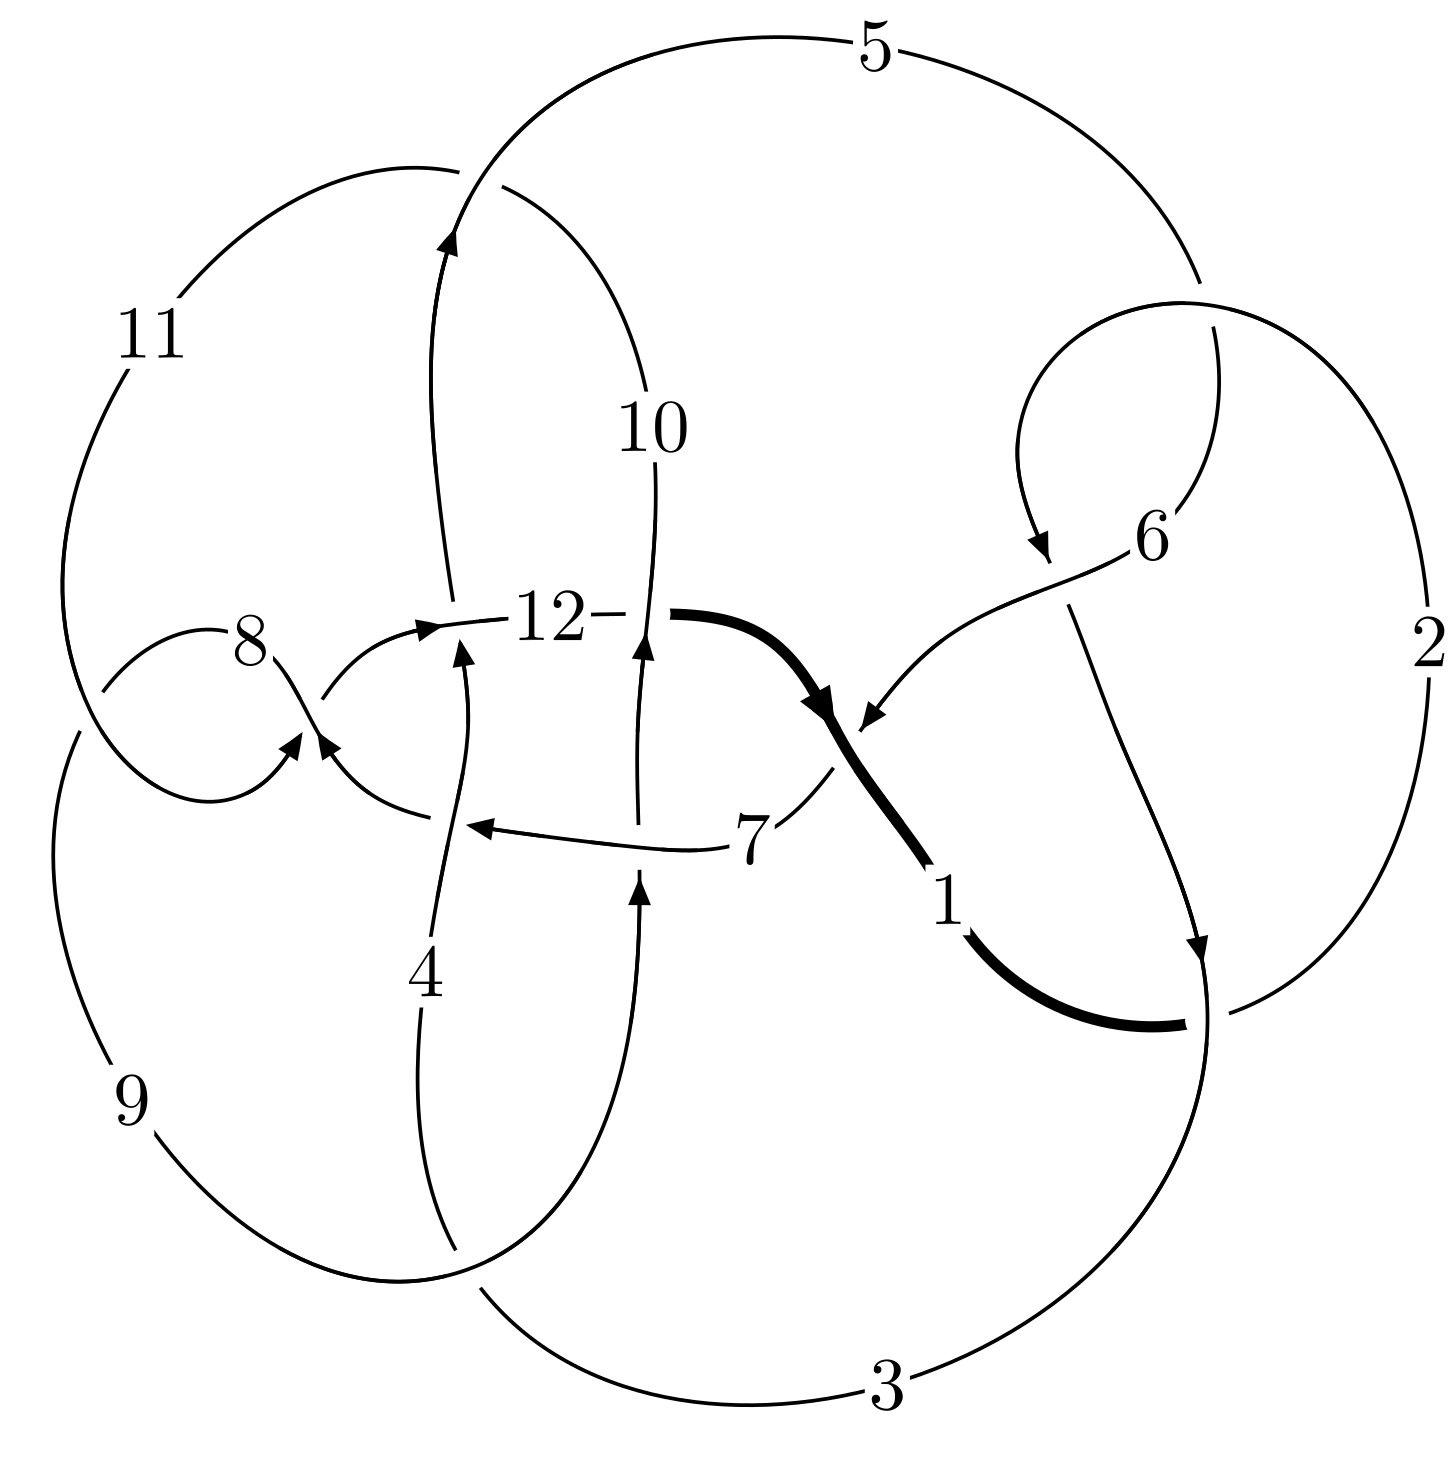
\includegraphics[width=112pt]{../../../GIT/diagram.site/Diagrams/png/1214_12a_0413.png}\\
\ \ \ A knot diagram\footnotemark}&
\allowdisplaybreaks
\textbf{Linearized knot diagam} \\
\cline{2-2}
 &
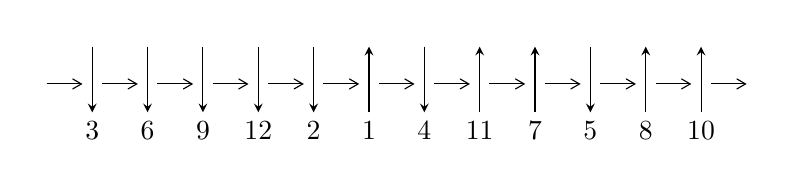
\begin{tikzpicture}[x=20pt, y=17pt]
	% nodes
	\node (C0) at (0, 0) {};
	\node (C1) at (1, 0) {};
	\node (C1U) at (1, +1) {};
	\node (C1D) at (1, -1) {3};

	\node (C2) at (2, 0) {};
	\node (C2U) at (2, +1) {};
	\node (C2D) at (2, -1) {6};

	\node (C3) at (3, 0) {};
	\node (C3U) at (3, +1) {};
	\node (C3D) at (3, -1) {9};

	\node (C4) at (4, 0) {};
	\node (C4U) at (4, +1) {};
	\node (C4D) at (4, -1) {12};

	\node (C5) at (5, 0) {};
	\node (C5U) at (5, +1) {};
	\node (C5D) at (5, -1) {2};

	\node (C6) at (6, 0) {};
	\node (C6U) at (6, +1) {};
	\node (C6D) at (6, -1) {1};

	\node (C7) at (7, 0) {};
	\node (C7U) at (7, +1) {};
	\node (C7D) at (7, -1) {4};

	\node (C8) at (8, 0) {};
	\node (C8U) at (8, +1) {};
	\node (C8D) at (8, -1) {11};

	\node (C9) at (9, 0) {};
	\node (C9U) at (9, +1) {};
	\node (C9D) at (9, -1) {7};

	\node (C10) at (10, 0) {};
	\node (C10U) at (10, +1) {};
	\node (C10D) at (10, -1) {5};

	\node (C11) at (11, 0) {};
	\node (C11U) at (11, +1) {};
	\node (C11D) at (11, -1) {8};

	\node (C12) at (12, 0) {};
	\node (C12U) at (12, +1) {};
	\node (C12D) at (12, -1) {10};
	\node (C13) at (13, 0) {};

	% arrows
	\draw[->,>={angle 60}]
	(C0) edge (C1) (C1) edge (C2) (C2) edge (C3) (C3) edge (C4) (C4) edge (C5) (C5) edge (C6) (C6) edge (C7) (C7) edge (C8) (C8) edge (C9) (C9) edge (C10) (C10) edge (C11) (C11) edge (C12) (C12) edge (C13) ;	\draw[->,>=stealth]
	(C1U) edge (C1D) (C2U) edge (C2D) (C3U) edge (C3D) (C4U) edge (C4D) (C5U) edge (C5D) (C6D) edge (C6U) (C7U) edge (C7D) (C8D) edge (C8U) (C9D) edge (C9U) (C10U) edge (C10D) (C11D) edge (C11U) (C12D) edge (C12U) ;
	\end{tikzpicture} \\
\hhline{~~} \\& 
\textbf{Solving Sequence} \\ \cline{2-2} 
 &
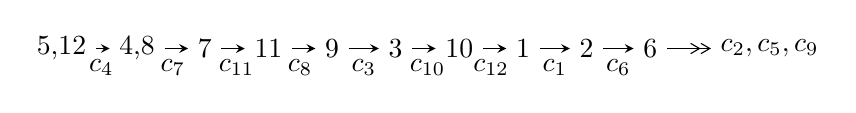
\begin{tikzpicture}[x=23pt, y=7pt]
	% node
	\node (A0) at (-1/8, 0) {5,12};
	\node (A1) at (17/16, 0) {4,8};
	\node (A2) at (17/8, 0) {7};
	\node (A3) at (25/8, 0) {11};
	\node (A4) at (33/8, 0) {9};
	\node (A5) at (41/8, 0) {3};
	\node (A6) at (49/8, 0) {10};
	\node (A7) at (57/8, 0) {1};
	\node (A8) at (65/8, 0) {2};
	\node (A9) at (73/8, 0) {6};
	\node (C1) at (1/2, -1) {$c_{4}$};
	\node (C2) at (13/8, -1) {$c_{7}$};
	\node (C3) at (21/8, -1) {$c_{11}$};
	\node (C4) at (29/8, -1) {$c_{8}$};
	\node (C5) at (37/8, -1) {$c_{3}$};
	\node (C6) at (45/8, -1) {$c_{10}$};
	\node (C7) at (53/8, -1) {$c_{12}$};
	\node (C8) at (61/8, -1) {$c_{1}$};
	\node (C9) at (69/8, -1) {$c_{6}$};
	\node (A10) at (11, 0) {$c_{2},c_{5},c_{9}$};

	% edge
	\draw[->,>=stealth]	
	(A0) edge (A1) (A1) edge (A2) (A2) edge (A3) (A3) edge (A4) (A4) edge (A5) (A5) edge (A6) (A6) edge (A7) (A7) edge (A8) (A8) edge (A9) ;
	\draw[->>,>={angle 60}]	
	(A9) edge (A10);
\end{tikzpicture} \\ 

\end{tabular} \\

\footnotetext{
The image of knot diagram is generated by the software ``\textbf{Draw programme}" developed by Andrew Bartholomew(\url{http://www.layer8.co.uk/maths/draw/index.htm\#Running-draw}), where we modified some parts for our purpose(\url{https://github.com/CATsTAILs/LinksPainter}).
}\phantom \\ \newline 
\centering \textbf{Ideals for irreducible components\footnotemark of $X_{\text{par}}$} 
 
\begin{align*}
I^u_{1}&=\langle 
-1.42965\times10^{227} u^{80}-1.46174\times10^{227} u^{79}+\cdots+3.55353\times10^{227} b-1.26641\times10^{227},\\
\phantom{I^u_{1}}&\phantom{= \langle  }3.52326\times10^{227} u^{80}+1.26641\times10^{227} u^{79}+\cdots+3.55353\times10^{227} a+1.44105\times10^{228},\;u^{81}-24 u^{79}+\cdots+5 u-1\rangle \\
I^u_{2}&=\langle 
1.14895\times10^{438} u^{95}-2.47031\times10^{438} u^{94}+\cdots+3.83896\times10^{439} b+6.50354\times10^{438},\\
\phantom{I^u_{2}}&\phantom{= \langle  }-2.04308\times10^{439} u^{95}+6.01402\times10^{439} u^{94}+\cdots+3.83896\times10^{439} a-8.80804\times10^{438},\\
\phantom{I^u_{2}}&\phantom{= \langle  }u^{96}-3 u^{95}+\cdots+16 u^2+2\rangle \\
I^u_{3}&=\langle 
-1.02996\times10^{27} u^{33}-6.93582\times10^{26} u^{32}+\cdots+5.98975\times10^{27} b+1.50476\times10^{27},\\
\phantom{I^u_{3}}&\phantom{= \langle  }-3.25125\times10^{27} u^{33}+1.50476\times10^{27} u^{32}+\cdots+5.98975\times10^{27} a+2.04748\times10^{27},\;u^{34}+6 u^{32}+\cdots- u+1\rangle \\
I^u_{4}&=\langle 
- u^3- u^2+b-1,\;u^3+2 u^2+2 a+u,\;u^4+2 u^3- u^2-2 u+2\rangle \\
\\
\end{align*}
\raggedright * 4 irreducible components of $\dim_{\mathbb{C}}=0$, with total 215 representations.\\
\footnotetext{All coefficients of polynomials are rational numbers. But the coefficients are sometimes approximated in decimal forms when there is not enough margin.}
\newpage
\renewcommand{\arraystretch}{1}
\centering \section*{I. $I^u_{1}= \langle -1.43\times10^{227} u^{80}-1.46\times10^{227} u^{79}+\cdots+3.55\times10^{227} b-1.27\times10^{227},\;3.52\times10^{227} u^{80}+1.27\times10^{227} u^{79}+\cdots+3.55\times10^{227} a+1.44\times10^{228},\;u^{81}-24 u^{79}+\cdots+5 u-1 \rangle$}
\flushleft \textbf{(i) Arc colorings}\\
\begin{tabular}{m{7pt} m{180pt} m{7pt} m{180pt} }
\flushright $a_{5}=$&$\begin{pmatrix}1\\0\end{pmatrix}$ \\
\flushright $a_{12}=$&$\begin{pmatrix}0\\u\end{pmatrix}$ \\
\flushright $a_{4}=$&$\begin{pmatrix}1\\- u^2\end{pmatrix}$ \\
\flushright $a_{8}=$&$\begin{pmatrix}-0.991483 u^{80}-0.356381 u^{79}+\cdots-65.8302 u-4.05525\\0.402319 u^{80}+0.411350 u^{79}+\cdots+0.209580 u+0.356381\end{pmatrix}$ \\
\flushright $a_{7}=$&$\begin{pmatrix}-0.991483 u^{80}-0.356381 u^{79}+\cdots-64.8302 u-4.05525\\0.402319 u^{80}+0.411350 u^{79}+\cdots+0.209580 u+0.356381\end{pmatrix}$ \\
\flushright $a_{11}=$&$\begin{pmatrix}1.07654 u^{80}+0.931549 u^{79}+\cdots-83.1510 u+0.150529\\-0.127897 u^{80}+0.0324780 u^{79}+\cdots+3.79078 u-0.575168\end{pmatrix}$ \\
\flushright $a_{9}=$&$\begin{pmatrix}2.59787 u^{80}+1.73504 u^{79}+\cdots-168.401 u+2.68154\\-0.947267 u^{80}-0.463794 u^{79}+\cdots+9.86812 u-2.31021\end{pmatrix}$ \\
\flushright $a_{3}=$&$\begin{pmatrix}-5.73123 u^{80}-1.06854 u^{79}+\cdots+39.9455 u-17.0848\\0.433762 u^{80}-0.169396 u^{79}+\cdots-3.97706 u+3.13069\end{pmatrix}$ \\
\flushright $a_{10}=$&$\begin{pmatrix}0.948644 u^{80}+0.964026 u^{79}+\cdots-79.3602 u-0.424639\\-0.127897 u^{80}+0.0324780 u^{79}+\cdots+3.79078 u-0.575168\end{pmatrix}$ \\
\flushright $a_{1}=$&$\begin{pmatrix}-2.13921 u^{80}-0.0773816 u^{79}+\cdots+95.7701 u-7.62114\\0.208044 u^{80}-0.323011 u^{79}+\cdots-3.13771 u+1.93467\end{pmatrix}$ \\
\flushright $a_{2}=$&$\begin{pmatrix}-12.5649 u^{80}-1.86559 u^{79}+\cdots-8.88741 u-70.4314\\0.506624 u^{80}+0.0528748 u^{79}+\cdots+9.81585 u+3.89395\end{pmatrix}$ \\
\flushright $a_{6}=$&$\begin{pmatrix}-16.1275 u^{80}-3.64845 u^{79}+\cdots-7.40160 u-63.9727\\1.38353 u^{80}+0.167871 u^{79}+\cdots+1.18482 u+6.65535\end{pmatrix}$\\&\end{tabular}
\flushleft \textbf{(ii) Obstruction class $= -1$}\\~\\
\flushleft \textbf{(iii) Cusp Shapes $= 4.39444 u^{80}+0.0171805 u^{79}+\cdots-42.0156 u+41.6462$}\\~\\
\newpage\renewcommand{\arraystretch}{1}
\flushleft \textbf{(iv) u-Polynomials at the component}\newline \\
\begin{tabular}{m{50pt}|m{274pt}}
Crossings & \hspace{64pt}u-Polynomials at each crossing \\
\hline $$\begin{aligned}c_{1}\end{aligned}$$&$\begin{aligned}
&u^{81}+40 u^{80}+\cdots+25 u+4
\end{aligned}$\\
\hline $$\begin{aligned}c_{2},c_{5}\end{aligned}$$&$\begin{aligned}
&u^{81}+8 u^{80}+\cdots+17 u+2
\end{aligned}$\\
\hline $$\begin{aligned}c_{3},c_{10}\end{aligned}$$&$\begin{aligned}
&u^{81}- u^{79}+\cdots-166 u+43
\end{aligned}$\\
\hline $$\begin{aligned}c_{4},c_{7}\end{aligned}$$&$\begin{aligned}
&u^{81}-24 u^{79}+\cdots+5 u+1
\end{aligned}$\\
\hline $$\begin{aligned}c_{6}\end{aligned}$$&$\begin{aligned}
&u^{81}+24 u^{80}+\cdots+358010 u+19264
\end{aligned}$\\
\hline $$\begin{aligned}c_{8},c_{11}\end{aligned}$$&$\begin{aligned}
&u^{81}+20 u^{80}+\cdots+11513 u+416
\end{aligned}$\\
\hline $$\begin{aligned}c_{9},c_{12}\end{aligned}$$&$\begin{aligned}
&u^{81}+2 u^{80}+\cdots+5 u+2
\end{aligned}$\\
\hline
\end{tabular}\\~\\
\newpage\renewcommand{\arraystretch}{1}
\flushleft \textbf{(v) Riley Polynomials at the component}\newline \\
\begin{tabular}{m{50pt}|m{274pt}}
Crossings & \hspace{64pt}Riley Polynomials at each crossing \\
\hline $$\begin{aligned}c_{1}\end{aligned}$$&$\begin{aligned}
&y^{81}+8 y^{80}+\cdots-239 y-16
\end{aligned}$\\
\hline $$\begin{aligned}c_{2},c_{5}\end{aligned}$$&$\begin{aligned}
&y^{81}-40 y^{80}+\cdots+25 y-4
\end{aligned}$\\
\hline $$\begin{aligned}c_{3},c_{10}\end{aligned}$$&$\begin{aligned}
&y^{81}-2 y^{80}+\cdots+40714 y-1849
\end{aligned}$\\
\hline $$\begin{aligned}c_{4},c_{7}\end{aligned}$$&$\begin{aligned}
&y^{81}-48 y^{80}+\cdots+141 y-1
\end{aligned}$\\
\hline $$\begin{aligned}c_{6}\end{aligned}$$&$\begin{aligned}
&y^{81}+24 y^{80}+\cdots+2334897828 y-371101696
\end{aligned}$\\
\hline $$\begin{aligned}c_{8},c_{11}\end{aligned}$$&$\begin{aligned}
&y^{81}+44 y^{80}+\cdots+10855025 y-173056
\end{aligned}$\\
\hline $$\begin{aligned}c_{9},c_{12}\end{aligned}$$&$\begin{aligned}
&y^{81}+44 y^{80}+\cdots-283 y-4
\end{aligned}$\\
\hline
\end{tabular}\\~\\
\newpage\flushleft \textbf{(vi) Complex Volumes and Cusp Shapes}
$$\begin{array}{c|c|c}  
\text{Solutions to }I^u_{1}& \I (\text{vol} + \sqrt{-1}CS) & \text{Cusp shape}\\
 \hline 
\begin{aligned}
u &= \phantom{-}0.903079 + 0.550850 I \\
a &= \phantom{-}0.429159 - 0.337361 I \\
b &= \phantom{-}0.347652 + 0.296638 I\end{aligned}
 & -1.95520 - 1.19929 I & \phantom{-0.000000 } 0 \\ \hline\begin{aligned}
u &= \phantom{-}0.903079 - 0.550850 I \\
a &= \phantom{-}0.429159 + 0.337361 I \\
b &= \phantom{-}0.347652 - 0.296638 I\end{aligned}
 & -1.95520 + 1.19929 I & \phantom{-0.000000 } 0 \\ \hline\begin{aligned}
u &= -1.083920 + 0.041793 I \\
a &= -0.579989 + 1.117260 I \\
b &= -0.50474 - 1.32145 I\end{aligned}
 & -8.88772 - 0.47155 I & \phantom{-0.000000 } 0 \\ \hline\begin{aligned}
u &= -1.083920 - 0.041793 I \\
a &= -0.579989 - 1.117260 I \\
b &= -0.50474 + 1.32145 I\end{aligned}
 & -8.88772 + 0.47155 I & \phantom{-0.000000 } 0 \\ \hline\begin{aligned}
u &= -0.878110 + 0.192771 I \\
a &= \phantom{-}0.12922 - 1.46095 I \\
b &= -0.478343 + 1.308730 I\end{aligned}
 & -3.72693 - 2.92513 I & \phantom{-0.000000 } 0 \\ \hline\begin{aligned}
u &= -0.878110 - 0.192771 I \\
a &= \phantom{-}0.12922 + 1.46095 I \\
b &= -0.478343 - 1.308730 I\end{aligned}
 & -3.72693 + 2.92513 I & \phantom{-0.000000 } 0 \\ \hline\begin{aligned}
u &= \phantom{-}0.893405 + 0.013006 I \\
a &= \phantom{-}0.43587 - 1.65249 I \\
b &= \phantom{-}0.50718 + 1.32157 I\end{aligned}
 & -10.03340 + 0.38814 I & \phantom{-0.000000 } 0 \\ \hline\begin{aligned}
u &= \phantom{-}0.893405 - 0.013006 I \\
a &= \phantom{-}0.43587 + 1.65249 I \\
b &= \phantom{-}0.50718 - 1.32157 I\end{aligned}
 & -10.03340 - 0.38814 I & \phantom{-0.000000 } 0 \\ \hline\begin{aligned}
u &= \phantom{-}0.969990 + 0.536933 I \\
a &= -0.460171 - 0.857076 I \\
b &= \phantom{-}0.37753 + 1.57558 I\end{aligned}
 & -3.51679 - 0.43160 I & \phantom{-0.000000 } 0 \\ \hline\begin{aligned}
u &= \phantom{-}0.969990 - 0.536933 I \\
a &= -0.460171 + 0.857076 I \\
b &= \phantom{-}0.37753 - 1.57558 I\end{aligned}
 & -3.51679 + 0.43160 I & \phantom{-0.000000 } 0\\
 \hline 
 \end{array}$$\newpage$$\begin{array}{c|c|c}  
\text{Solutions to }I^u_{1}& \I (\text{vol} + \sqrt{-1}CS) & \text{Cusp shape}\\
 \hline 
\begin{aligned}
u &= -1.006130 + 0.470317 I \\
a &= -0.293775 - 0.438445 I \\
b &= -0.358781 + 0.539142 I\end{aligned}
 & -4.68916 - 3.35217 I & \phantom{-0.000000 } 0 \\ \hline\begin{aligned}
u &= -1.006130 - 0.470317 I \\
a &= -0.293775 + 0.438445 I \\
b &= -0.358781 - 0.539142 I\end{aligned}
 & -4.68916 + 3.35217 I & \phantom{-0.000000 } 0 \\ \hline\begin{aligned}
u &= -0.861433 + 0.051722 I \\
a &= -0.26645 - 1.73774 I \\
b &= -0.509575 + 1.312850 I\end{aligned}
 & -5.94203 - 3.76063 I & \phantom{-0.000000 } 0 \\ \hline\begin{aligned}
u &= -0.861433 - 0.051722 I \\
a &= -0.26645 + 1.73774 I \\
b &= -0.509575 - 1.312850 I\end{aligned}
 & -5.94203 + 3.76063 I & \phantom{-0.000000 } 0 \\ \hline\begin{aligned}
u &= -0.980345 + 0.615042 I \\
a &= -0.518246 - 0.465904 I \\
b &= -0.116475 + 0.261615 I\end{aligned}
 & -5.91291 + 4.69549 I & \phantom{-0.000000 } 0 \\ \hline\begin{aligned}
u &= -0.980345 - 0.615042 I \\
a &= -0.518246 + 0.465904 I \\
b &= -0.116475 - 0.261615 I\end{aligned}
 & -5.91291 - 4.69549 I & \phantom{-0.000000 } 0 \\ \hline\begin{aligned}
u &= \phantom{-}0.839001 + 0.031227 I \\
a &= \phantom{-}0.32065 - 1.84947 I \\
b &= \phantom{-}0.516689 + 1.314510 I\end{aligned}
 & -8.62816 + 8.54082 I & \phantom{-0.000000 } 0 \\ \hline\begin{aligned}
u &= \phantom{-}0.839001 - 0.031227 I \\
a &= \phantom{-}0.32065 + 1.84947 I \\
b &= \phantom{-}0.516689 - 1.314510 I\end{aligned}
 & -8.62816 - 8.54082 I & \phantom{-0.000000 } 0 \\ \hline\begin{aligned}
u &= \phantom{-}1.162140 + 0.230832 I \\
a &= \phantom{-}0.156751 - 0.894141 I \\
b &= \phantom{-}0.479067 + 1.306700 I\end{aligned}
 & -3.03442 - 0.89093 I & \phantom{-0.000000 } 0 \\ \hline\begin{aligned}
u &= \phantom{-}1.162140 - 0.230832 I \\
a &= \phantom{-}0.156751 + 0.894141 I \\
b &= \phantom{-}0.479067 - 1.306700 I\end{aligned}
 & -3.03442 + 0.89093 I & \phantom{-0.000000 } 0\\
 \hline 
 \end{array}$$\newpage$$\begin{array}{c|c|c}  
\text{Solutions to }I^u_{1}& \I (\text{vol} + \sqrt{-1}CS) & \text{Cusp shape}\\
 \hline 
\begin{aligned}
u &= -0.970022 + 0.698699 I \\
a &= -0.805602 - 0.341776 I \\
b &= -0.141996 - 0.238556 I\end{aligned}
 & \phantom{-}1.96549 + 7.02940 I & \phantom{-0.000000 } 0 \\ \hline\begin{aligned}
u &= -0.970022 - 0.698699 I \\
a &= -0.805602 + 0.341776 I \\
b &= -0.141996 + 0.238556 I\end{aligned}
 & \phantom{-}1.96549 - 7.02940 I & \phantom{-0.000000 } 0 \\ \hline\begin{aligned}
u &= \phantom{-}0.960828 + 0.712083 I \\
a &= \phantom{-}0.753196 - 0.275712 I \\
b &= \phantom{-}0.270124 - 0.203842 I\end{aligned}
 & \phantom{-}1.55787 - 1.96344 I & \phantom{-0.000000 } 0 \\ \hline\begin{aligned}
u &= \phantom{-}0.960828 - 0.712083 I \\
a &= \phantom{-}0.753196 + 0.275712 I \\
b &= \phantom{-}0.270124 + 0.203842 I\end{aligned}
 & \phantom{-}1.55787 + 1.96344 I & \phantom{-0.000000 } 0 \\ \hline\begin{aligned}
u &= -1.141990 + 0.355379 I \\
a &= -0.022029 - 0.642644 I \\
b &= -0.594423 + 1.094440 I\end{aligned}
 & -4.74824 - 3.47457 I & \phantom{-0.000000 } 0 \\ \hline\begin{aligned}
u &= -1.141990 - 0.355379 I \\
a &= -0.022029 + 0.642644 I \\
b &= -0.594423 - 1.094440 I\end{aligned}
 & -4.74824 + 3.47457 I & \phantom{-0.000000 } 0 \\ \hline\begin{aligned}
u &= -0.974870 + 0.694526 I \\
a &= -0.843489 - 0.462950 I \\
b &= \phantom{-}0.046789 - 0.231017 I\end{aligned}
 & -0.32356 + 9.29303 I & \phantom{-0.000000 } 0 \\ \hline\begin{aligned}
u &= -0.974870 - 0.694526 I \\
a &= -0.843489 + 0.462950 I \\
b &= \phantom{-}0.046789 + 0.231017 I\end{aligned}
 & -0.32356 - 9.29303 I & \phantom{-0.000000 } 0 \\ \hline\begin{aligned}
u &= \phantom{-}0.978304 + 0.690962 I \\
a &= \phantom{-}0.785381 - 0.489695 I \\
b &= -0.060443 - 0.135945 I\end{aligned}
 & -4.99194 - 6.09651 I & \phantom{-0.000000 } 0 \\ \hline\begin{aligned}
u &= \phantom{-}0.978304 - 0.690962 I \\
a &= \phantom{-}0.785381 + 0.489695 I \\
b &= -0.060443 + 0.135945 I\end{aligned}
 & -4.99194 + 6.09651 I & \phantom{-0.000000 } 0\\
 \hline 
 \end{array}$$\newpage$$\begin{array}{c|c|c}  
\text{Solutions to }I^u_{1}& \I (\text{vol} + \sqrt{-1}CS) & \text{Cusp shape}\\
 \hline 
\begin{aligned}
u &= \phantom{-}0.975319 + 0.696384 I \\
a &= \phantom{-}0.862768 - 0.491837 I \\
b &= -0.095096 - 0.246252 I\end{aligned}
 & -2.8881 - 14.4050 I & \phantom{-0.000000 } 0 \\ \hline\begin{aligned}
u &= \phantom{-}0.975319 - 0.696384 I \\
a &= \phantom{-}0.862768 + 0.491837 I \\
b &= -0.095096 + 0.246252 I\end{aligned}
 & -2.8881 + 14.4050 I & \phantom{-0.000000 } 0 \\ \hline\begin{aligned}
u &= -1.200610 + 0.135296 I \\
a &= -0.663574 + 0.864477 I \\
b &= -0.53709 - 1.31057 I\end{aligned}
 & -6.37178 - 8.44892 I & \phantom{-0.000000 } 0 \\ \hline\begin{aligned}
u &= -1.200610 - 0.135296 I \\
a &= -0.663574 - 0.864477 I \\
b &= -0.53709 + 1.31057 I\end{aligned}
 & -6.37178 + 8.44892 I & \phantom{-0.000000 } 0 \\ \hline\begin{aligned}
u &= \phantom{-}1.219070 + 0.053782 I \\
a &= \phantom{-}0.544832 + 0.888452 I \\
b &= \phantom{-}0.52746 - 1.33544 I\end{aligned}
 & -4.07346 + 3.22609 I & \phantom{-0.000000 } 0 \\ \hline\begin{aligned}
u &= \phantom{-}1.219070 - 0.053782 I \\
a &= \phantom{-}0.544832 - 0.888452 I \\
b &= \phantom{-}0.52746 + 1.33544 I\end{aligned}
 & -4.07346 - 3.22609 I & \phantom{-0.000000 } 0 \\ \hline\begin{aligned}
u &= -1.169330 + 0.379709 I \\
a &= \phantom{-}0.231493 - 0.620798 I \\
b &= -0.90121 + 1.34461 I\end{aligned}
 & -5.09366 + 3.39097 I & \phantom{-0.000000 } 0 \\ \hline\begin{aligned}
u &= -1.169330 - 0.379709 I \\
a &= \phantom{-}0.231493 + 0.620798 I \\
b &= -0.90121 - 1.34461 I\end{aligned}
 & -5.09366 - 3.39097 I & \phantom{-0.000000 } 0 \\ \hline\begin{aligned}
u &= \phantom{-}1.152460 + 0.435758 I \\
a &= -0.305450 - 0.699799 I \\
b &= \phantom{-}0.79728 + 1.53911 I\end{aligned}
 & -3.10119 + 0.19958 I & \phantom{-0.000000 } 0 \\ \hline\begin{aligned}
u &= \phantom{-}1.152460 - 0.435758 I \\
a &= -0.305450 + 0.699799 I \\
b &= \phantom{-}0.79728 - 1.53911 I\end{aligned}
 & -3.10119 - 0.19958 I & \phantom{-0.000000 } 0\\
 \hline 
 \end{array}$$\newpage$$\begin{array}{c|c|c}  
\text{Solutions to }I^u_{1}& \I (\text{vol} + \sqrt{-1}CS) & \text{Cusp shape}\\
 \hline 
\begin{aligned}
u &= \phantom{-}0.613617 + 0.423176 I \\
a &= -1.03569 - 1.08690 I \\
b &= \phantom{-}0.253643 + 1.175650 I\end{aligned}
 & -3.80121 - 0.19494 I & \phantom{-0.000000 } 0 \\ \hline\begin{aligned}
u &= \phantom{-}0.613617 - 0.423176 I \\
a &= -1.03569 + 1.08690 I \\
b &= \phantom{-}0.253643 - 1.175650 I\end{aligned}
 & -3.80121 + 0.19494 I & \phantom{-0.000000 } 0 \\ \hline\begin{aligned}
u &= \phantom{-}1.158590 + 0.508165 I \\
a &= -0.384496 - 0.720116 I \\
b &= \phantom{-}0.72748 + 1.74159 I\end{aligned}
 & -3.49408 + 0.28112 I & \phantom{-0.000000 } 0 \\ \hline\begin{aligned}
u &= \phantom{-}1.158590 - 0.508165 I \\
a &= -0.384496 + 0.720116 I \\
b &= \phantom{-}0.72748 - 1.74159 I\end{aligned}
 & -3.49408 - 0.28112 I & \phantom{-0.000000 } 0 \\ \hline\begin{aligned}
u &= -1.173590 + 0.570860 I \\
a &= \phantom{-}0.427375 - 0.725476 I \\
b &= -0.65087 + 1.90628 I\end{aligned}
 & -6.45309 + 3.20546 I & \phantom{-0.000000 } 0 \\ \hline\begin{aligned}
u &= -1.173590 - 0.570860 I \\
a &= \phantom{-}0.427375 + 0.725476 I \\
b &= -0.65087 - 1.90628 I\end{aligned}
 & -6.45309 - 3.20546 I & \phantom{-0.000000 } 0 \\ \hline\begin{aligned}
u &= -1.202720 + 0.521369 I \\
a &= \phantom{-}0.409907 - 0.693687 I \\
b &= -0.81427 + 1.85032 I\end{aligned}
 & -6.07010 - 4.33648 I & \phantom{-0.000000 } 0 \\ \hline\begin{aligned}
u &= -1.202720 - 0.521369 I \\
a &= \phantom{-}0.409907 + 0.693687 I \\
b &= -0.81427 - 1.85032 I\end{aligned}
 & -6.07010 + 4.33648 I & \phantom{-0.000000 } 0 \\ \hline\begin{aligned}
u &= -0.13101 + 1.42903 I \\
a &= \phantom{-}0.507329 - 0.241819 I \\
b &= \phantom{-}0.98685 + 1.12932 I\end{aligned}
 & \phantom{-}2.74929 - 1.56105 I & \phantom{-0.000000 } 0 \\ \hline\begin{aligned}
u &= -0.13101 - 1.42903 I \\
a &= \phantom{-}0.507329 + 0.241819 I \\
b &= \phantom{-}0.98685 - 1.12932 I\end{aligned}
 & \phantom{-}2.74929 + 1.56105 I & \phantom{-0.000000 } 0\\
 \hline 
 \end{array}$$\newpage$$\begin{array}{c|c|c}  
\text{Solutions to }I^u_{1}& \I (\text{vol} + \sqrt{-1}CS) & \text{Cusp shape}\\
 \hline 
\begin{aligned}
u &= -0.397723 + 0.375405 I \\
a &= \phantom{-}1.72040 - 0.69997 I \\
b &= -0.218386 + 0.901221 I\end{aligned}
 & \phantom{-}0.03236 - 2.49515 I & \phantom{-}0.44371 + 2.70738 I \\ \hline\begin{aligned}
u &= -0.397723 - 0.375405 I \\
a &= \phantom{-}1.72040 + 0.69997 I \\
b &= -0.218386 - 0.901221 I\end{aligned}
 & \phantom{-}0.03236 + 2.49515 I & \phantom{-}0.44371 - 2.70738 I \\ \hline\begin{aligned}
u &= \phantom{-}0.444303 + 0.311469 I \\
a &= -1.84853 - 1.09502 I \\
b &= \phantom{-}0.326808 + 0.933026 I\end{aligned}
 & -2.33464 + 7.11407 I & -3.06794 - 6.14015 I \\ \hline\begin{aligned}
u &= \phantom{-}0.444303 - 0.311469 I \\
a &= -1.84853 + 1.09502 I \\
b &= \phantom{-}0.326808 - 0.933026 I\end{aligned}
 & -2.33464 - 7.11407 I & -3.06794 + 6.14015 I \\ \hline\begin{aligned}
u &= \phantom{-}0.456913\phantom{ +0.000000I} \\
a &= \phantom{-}0.253678\phantom{ +0.000000I} \\
b &= \phantom{-}0.403953\phantom{ +0.000000I}\end{aligned}
 & -0.942905\phantom{ +0.000000I} & -11.1650\phantom{ +0.000000I} \\ \hline\begin{aligned}
u &= \phantom{-}0.51889 + 1.52238 I \\
a &= -0.446848 - 0.338033 I \\
b &= -0.93049 + 1.53593 I\end{aligned}
 & \phantom{-}2.46516 - 4.28325 I & \phantom{-0.000000 } 0 \\ \hline\begin{aligned}
u &= \phantom{-}0.51889 - 1.52238 I \\
a &= -0.446848 + 0.338033 I \\
b &= -0.93049 - 1.53593 I\end{aligned}
 & \phantom{-}2.46516 + 4.28325 I & \phantom{-0.000000 } 0 \\ \hline\begin{aligned}
u &= -1.28578 + 1.02589 I \\
a &= \phantom{-}0.300936 - 0.698163 I \\
b &= \phantom{-}0.37528 + 2.23926 I\end{aligned}
 & -8.73798 - 0.20568 I & \phantom{-0.000000 } 0 \\ \hline\begin{aligned}
u &= -1.28578 - 1.02589 I \\
a &= \phantom{-}0.300936 + 0.698163 I \\
b &= \phantom{-}0.37528 - 2.23926 I\end{aligned}
 & -8.73798 + 0.20568 I & \phantom{-0.000000 } 0 \\ \hline\begin{aligned}
u &= -0.172413 + 0.277440 I \\
a &= \phantom{-}2.25399 + 0.95734 I \\
b &= -0.157507 + 0.538306 I\end{aligned}
 & \phantom{-}1.32239 - 1.55771 I & \phantom{-}2.58702 + 5.50475 I\\
 \hline 
 \end{array}$$\newpage$$\begin{array}{c|c|c}  
\text{Solutions to }I^u_{1}& \I (\text{vol} + \sqrt{-1}CS) & \text{Cusp shape}\\
 \hline 
\begin{aligned}
u &= -0.172413 - 0.277440 I \\
a &= \phantom{-}2.25399 - 0.95734 I \\
b &= -0.157507 - 0.538306 I\end{aligned}
 & \phantom{-}1.32239 + 1.55771 I & \phantom{-}2.58702 - 5.50475 I \\ \hline\begin{aligned}
u &= \phantom{-}1.39144 + 0.93444 I \\
a &= -0.151774 - 0.865162 I \\
b &= -0.69703 + 2.24874 I\end{aligned}
 & -6.7665 - 20.6415 I & \phantom{-0.000000 } 0 \\ \hline\begin{aligned}
u &= \phantom{-}1.39144 - 0.93444 I \\
a &= -0.151774 + 0.865162 I \\
b &= -0.69703 - 2.24874 I\end{aligned}
 & -6.7665 + 20.6415 I & \phantom{-0.000000 } 0 \\ \hline\begin{aligned}
u &= -1.39492 + 0.93638 I \\
a &= \phantom{-}0.148970 - 0.852295 I \\
b &= \phantom{-}0.67232 + 2.23665 I\end{aligned}
 & -4.0945 + 15.3933 I & \phantom{-0.000000 } 0 \\ \hline\begin{aligned}
u &= -1.39492 - 0.93638 I \\
a &= \phantom{-}0.148970 + 0.852295 I \\
b &= \phantom{-}0.67232 - 2.23665 I\end{aligned}
 & -4.0945 - 15.3933 I & \phantom{-0.000000 } 0 \\ \hline\begin{aligned}
u &= \phantom{-}1.39156 + 0.94333 I \\
a &= -0.170590 - 0.842332 I \\
b &= -0.64135 + 2.27276 I\end{aligned}
 & -8.9687 - 11.9497 I & \phantom{-0.000000 } 0 \\ \hline\begin{aligned}
u &= \phantom{-}1.39156 - 0.94333 I \\
a &= -0.170590 + 0.842332 I \\
b &= -0.64135 - 2.27276 I\end{aligned}
 & -8.9687 + 11.9497 I & \phantom{-0.000000 } 0 \\ \hline\begin{aligned}
u &= -1.35748 + 0.99485 I \\
a &= \phantom{-}0.243220 - 0.748871 I \\
b &= \phantom{-}0.45774 + 2.29058 I\end{aligned}
 & -10.01880 + 8.98125 I & \phantom{-0.000000 } 0 \\ \hline\begin{aligned}
u &= -1.35748 - 0.99485 I \\
a &= \phantom{-}0.243220 + 0.748871 I \\
b &= \phantom{-}0.45774 - 2.29058 I\end{aligned}
 & -10.01880 - 8.98125 I & \phantom{-0.000000 } 0 \\ \hline\begin{aligned}
u &= \phantom{-}1.34234 + 1.04798 I \\
a &= -0.250789 - 0.693209 I \\
b &= -0.43153 + 2.24133 I\end{aligned}
 & -5.50274 - 4.90115 I & \phantom{-0.000000 } 0\\
 \hline 
 \end{array}$$\newpage$$\begin{array}{c|c|c}  
\text{Solutions to }I^u_{1}& \I (\text{vol} + \sqrt{-1}CS) & \text{Cusp shape}\\
 \hline 
\begin{aligned}
u &= \phantom{-}1.34234 - 1.04798 I \\
a &= -0.250789 + 0.693209 I \\
b &= -0.43153 - 2.24133 I\end{aligned}
 & -5.50274 + 4.90115 I & \phantom{-0.000000 } 0 \\ \hline\begin{aligned}
u &= -1.41876 + 0.94350 I \\
a &= \phantom{-}0.124214 - 0.801178 I \\
b &= \phantom{-}0.58669 + 2.17551 I\end{aligned}
 & -1.24782 + 12.75560 I & \phantom{-0.000000 } 0 \\ \hline\begin{aligned}
u &= -1.41876 - 0.94350 I \\
a &= \phantom{-}0.124214 + 0.801178 I \\
b &= \phantom{-}0.58669 - 2.17551 I\end{aligned}
 & -1.24782 - 12.75560 I & \phantom{-0.000000 } 0 \\ \hline\begin{aligned}
u &= \phantom{-}1.43602 + 0.96116 I \\
a &= -0.124783 - 0.763025 I \\
b &= -0.52826 + 2.17418 I\end{aligned}
 & -1.39931 - 7.33732 I & \phantom{-0.000000 } 0 \\ \hline\begin{aligned}
u &= \phantom{-}1.43602 - 0.96116 I \\
a &= -0.124783 + 0.763025 I \\
b &= -0.52826 - 2.17418 I\end{aligned}
 & -1.39931 + 7.33732 I & \phantom{-0.000000 } 0 \\ \hline\begin{aligned}
u &= \phantom{-}0.191879 + 0.136262 I \\
a &= -4.57848 + 1.23371 I \\
b &= \phantom{-}0.339950 + 0.353163 I\end{aligned}
 & \phantom{-}0.04190 - 2.04058 I & \phantom{-}2.67481 + 0.29939 I \\ \hline\begin{aligned}
u &= \phantom{-}0.191879 - 0.136262 I \\
a &= -4.57848 - 1.23371 I \\
b &= \phantom{-}0.339950 - 0.353163 I\end{aligned}
 & \phantom{-}0.04190 + 2.04058 I & \phantom{-}2.67481 - 0.29939 I \\ \hline\begin{aligned}
u &= \phantom{-}0.199528 + 0.058202 I \\
a &= -6.15885 + 0.67502 I \\
b &= \phantom{-}0.439537 + 0.176661 I\end{aligned}
 & \phantom{-}0.60362 + 4.61374 I & \phantom{-}6.36261 - 6.48089 I \\ \hline\begin{aligned}
u &= \phantom{-}0.199528 - 0.058202 I \\
a &= -6.15885 - 0.67502 I \\
b &= \phantom{-}0.439537 - 0.176661 I\end{aligned}
 & \phantom{-}0.60362 - 4.61374 I & \phantom{-}6.36261 + 6.48089 I \\ \hline\begin{aligned}
u &= -0.169065 + 0.033618 I \\
a &= \phantom{-}6.99710 + 0.79348 I \\
b &= -0.370174 + 0.091371 I\end{aligned}
 & \phantom{-}2.60987 - 0.42182 I & \phantom{-}12.11739 + 2.00022 I\\
 \hline 
 \end{array}$$\newpage$$\begin{array}{c|c|c}  
\text{Solutions to }I^u_{1}& \I (\text{vol} + \sqrt{-1}CS) & \text{Cusp shape}\\
 \hline 
\begin{aligned}
u &= -0.169065 - 0.033618 I \\
a &= \phantom{-}6.99710 - 0.79348 I \\
b &= -0.370174 - 0.091371 I\end{aligned}
 & \phantom{-}2.60987 + 0.42182 I & \phantom{-}12.11739 - 2.00022 I\\
 \hline 
 \end{array}$$\newpage\newpage\renewcommand{\arraystretch}{1}
\centering \section*{II. $I^u_{2}= \langle 1.15\times10^{438} u^{95}-2.47\times10^{438} u^{94}+\cdots+3.84\times10^{439} b+6.50\times10^{438},\;-2.04\times10^{439} u^{95}+6.01\times10^{439} u^{94}+\cdots+3.84\times10^{439} a-8.81\times10^{438},\;u^{96}-3 u^{95}+\cdots+16 u^2+2 \rangle$}
\flushleft \textbf{(i) Arc colorings}\\
\begin{tabular}{m{7pt} m{180pt} m{7pt} m{180pt} }
\flushright $a_{5}=$&$\begin{pmatrix}1\\0\end{pmatrix}$ \\
\flushright $a_{12}=$&$\begin{pmatrix}0\\u\end{pmatrix}$ \\
\flushright $a_{4}=$&$\begin{pmatrix}1\\- u^2\end{pmatrix}$ \\
\flushright $a_{8}=$&$\begin{pmatrix}0.532197 u^{95}-1.56658 u^{94}+\cdots+8.79516 u+0.229438\\-0.0299288 u^{95}+0.0643484 u^{94}+\cdots+0.269231 u-0.169409\end{pmatrix}$ \\
\flushright $a_{7}=$&$\begin{pmatrix}\frac{1}{2} u^{95}-\frac{3}{2} u^{94}+\cdots-\frac{41}{2} u^2+8 u\\-0.0321972 u^{95}+0.0665767 u^{94}+\cdots+0.204837 u-0.229438\end{pmatrix}$ \\
\flushright $a_{11}=$&$\begin{pmatrix}0.575081 u^{95}-1.66673 u^{94}+\cdots+9.69187 u+0.527136\\-0.0360635 u^{95}+0.0883803 u^{94}+\cdots+1.25346 u-0.180674\end{pmatrix}$ \\
\flushright $a_{9}=$&$\begin{pmatrix}1.15647 u^{95}-3.35032 u^{94}+\cdots+19.4650 u+1.10864\\-0.0633405 u^{95}+0.149731 u^{94}+\cdots+1.60421 u-0.283309\end{pmatrix}$ \\
\flushright $a_{3}=$&$\begin{pmatrix}0.609013 u^{95}-1.98147 u^{94}+\cdots+10.7863 u-0.679440\\0.144780 u^{95}-0.460723 u^{94}+\cdots+1.48348 u-0.352848\end{pmatrix}$ \\
\flushright $a_{10}=$&$\begin{pmatrix}0.539018 u^{95}-1.57835 u^{94}+\cdots+10.9453 u+0.346462\\-0.0360635 u^{95}+0.0883803 u^{94}+\cdots+1.25346 u-0.180674\end{pmatrix}$ \\
\flushright $a_{1}=$&$\begin{pmatrix}-0.624301 u^{95}+1.78526 u^{94}+\cdots-14.3857 u-1.06687\\0.0271219 u^{95}-0.0569288 u^{94}+\cdots-0.226824 u+0.185505\end{pmatrix}$ \\
\flushright $a_{2}=$&$\begin{pmatrix}-0.240992 u^{95}+0.679703 u^{94}+\cdots-7.35020 u-1.71513\\-0.129481 u^{95}+0.427106 u^{94}+\cdots-0.741908 u+0.241757\end{pmatrix}$ \\
\flushright $a_{6}=$&$\begin{pmatrix}0.107195 u^{95}-0.543300 u^{94}+\cdots+1.75034 u-3.48636\\-0.142490 u^{95}+0.417692 u^{94}+\cdots-0.328294 u-0.440229\end{pmatrix}$\\&\end{tabular}
\flushleft \textbf{(ii) Obstruction class $= -1$}\\~\\
\flushleft \textbf{(iii) Cusp Shapes $= 1.18779 u^{95}-3.29337 u^{94}+\cdots+3.37341 u+9.33011$}\\~\\
\newpage\renewcommand{\arraystretch}{1}
\flushleft \textbf{(iv) u-Polynomials at the component}\newline \\
\begin{tabular}{m{50pt}|m{274pt}}
Crossings & \hspace{64pt}u-Polynomials at each crossing \\
\hline $$\begin{aligned}c_{1}\end{aligned}$$&$\begin{aligned}
&(u^{48}+25 u^{47}+\cdots+3 u+1)^{2}
\end{aligned}$\\
\hline $$\begin{aligned}c_{2},c_{5}\end{aligned}$$&$\begin{aligned}
&(u^{48}-3 u^{47}+\cdots-3 u+1)^{2}
\end{aligned}$\\
\hline $$\begin{aligned}c_{3},c_{10}\end{aligned}$$&$\begin{aligned}
&u^{96}- u^{95}+\cdots+3112 u+446
\end{aligned}$\\
\hline $$\begin{aligned}c_{4},c_{7}\end{aligned}$$&$\begin{aligned}
&u^{96}+3 u^{95}+\cdots+16 u^2+2
\end{aligned}$\\
\hline $$\begin{aligned}c_{6}\end{aligned}$$&$\begin{aligned}
&(u^{48}-15 u^{47}+\cdots-536 u+48)^{2}
\end{aligned}$\\
\hline $$\begin{aligned}c_{8},c_{11}\end{aligned}$$&$\begin{aligned}
&(u^{48}-15 u^{47}+\cdots-19 u+3)^{2}
\end{aligned}$\\
\hline $$\begin{aligned}c_{9},c_{12}\end{aligned}$$&$\begin{aligned}
&u^{96}+15 u^{95}+\cdots+380 u+113
\end{aligned}$\\
\hline
\end{tabular}\\~\\
\newpage\renewcommand{\arraystretch}{1}
\flushleft \textbf{(v) Riley Polynomials at the component}\newline \\
\begin{tabular}{m{50pt}|m{274pt}}
Crossings & \hspace{64pt}Riley Polynomials at each crossing \\
\hline $$\begin{aligned}c_{1}\end{aligned}$$&$\begin{aligned}
&(y^{48}- y^{47}+\cdots+21 y+1)^{2}
\end{aligned}$\\
\hline $$\begin{aligned}c_{2},c_{5}\end{aligned}$$&$\begin{aligned}
&(y^{48}-25 y^{47}+\cdots-3 y+1)^{2}
\end{aligned}$\\
\hline $$\begin{aligned}c_{3},c_{10}\end{aligned}$$&$\begin{aligned}
&y^{96}-15 y^{95}+\cdots-3527960 y+198916
\end{aligned}$\\
\hline $$\begin{aligned}c_{4},c_{7}\end{aligned}$$&$\begin{aligned}
&y^{96}+9 y^{95}+\cdots+64 y+4
\end{aligned}$\\
\hline $$\begin{aligned}c_{6}\end{aligned}$$&$\begin{aligned}
&(y^{48}+21 y^{47}+\cdots-2752 y+2304)^{2}
\end{aligned}$\\
\hline $$\begin{aligned}c_{8},c_{11}\end{aligned}$$&$\begin{aligned}
&(y^{48}+31 y^{47}+\cdots+281 y+9)^{2}
\end{aligned}$\\
\hline $$\begin{aligned}c_{9},c_{12}\end{aligned}$$&$\begin{aligned}
&y^{96}-21 y^{95}+\cdots-876866 y+12769
\end{aligned}$\\
\hline
\end{tabular}\\~\\
\newpage\flushleft \textbf{(vi) Complex Volumes and Cusp Shapes}
$$\begin{array}{c|c|c}  
\text{Solutions to }I^u_{2}& \I (\text{vol} + \sqrt{-1}CS) & \text{Cusp shape}\\
 \hline 
\begin{aligned}
u &= -0.642886 + 0.769233 I \\
a &= -0.526834 + 1.245750 I \\
b &= -0.159604 - 0.779166 I\end{aligned}
 & -2.64526 + 1.62822 I & \phantom{-0.000000 } 0 \\ \hline\begin{aligned}
u &= -0.642886 - 0.769233 I \\
a &= -0.526834 - 1.245750 I \\
b &= -0.159604 + 0.779166 I\end{aligned}
 & -2.64526 - 1.62822 I & \phantom{-0.000000 } 0 \\ \hline\begin{aligned}
u &= -0.881612 + 0.504458 I \\
a &= -0.284621 + 1.359290 I \\
b &= \phantom{-}0.07887 - 1.83409 I\end{aligned}
 & -3.39889 + 6.05165 I & \phantom{-0.000000 } 0 \\ \hline\begin{aligned}
u &= -0.881612 - 0.504458 I \\
a &= -0.284621 - 1.359290 I \\
b &= \phantom{-}0.07887 + 1.83409 I\end{aligned}
 & -3.39889 - 6.05165 I & \phantom{-0.000000 } 0 \\ \hline\begin{aligned}
u &= -0.550537 + 0.862614 I \\
a &= -0.353146 + 0.068121 I \\
b &= \phantom{-}0.658429 + 0.450242 I\end{aligned}
 & -4.39871 + 0.53615 I & \phantom{-0.000000 } 0 \\ \hline\begin{aligned}
u &= -0.550537 - 0.862614 I \\
a &= -0.353146 - 0.068121 I \\
b &= \phantom{-}0.658429 - 0.450242 I\end{aligned}
 & -4.39871 - 0.53615 I & \phantom{-0.000000 } 0 \\ \hline\begin{aligned}
u &= \phantom{-}0.591865 + 0.735838 I \\
a &= -0.530706 - 0.763908 I \\
b &= -0.89983 + 1.90530 I\end{aligned}
 & \phantom{-}2.33675 - 3.85987 I & \phantom{-0.000000 } 0 \\ \hline\begin{aligned}
u &= \phantom{-}0.591865 - 0.735838 I \\
a &= -0.530706 + 0.763908 I \\
b &= -0.89983 - 1.90530 I\end{aligned}
 & \phantom{-}2.33675 + 3.85987 I & \phantom{-0.000000 } 0 \\ \hline\begin{aligned}
u &= \phantom{-}0.744875 + 0.808215 I \\
a &= \phantom{-}0.499652 + 1.192210 I \\
b &= \phantom{-}0.368377 - 1.007510 I\end{aligned}
 & -1.16841 - 5.60646 I & \phantom{-0.000000 } 0 \\ \hline\begin{aligned}
u &= \phantom{-}0.744875 - 0.808215 I \\
a &= \phantom{-}0.499652 - 1.192210 I \\
b &= \phantom{-}0.368377 + 1.007510 I\end{aligned}
 & -1.16841 + 5.60646 I & \phantom{-0.000000 } 0\\
 \hline 
 \end{array}$$\newpage$$\begin{array}{c|c|c}  
\text{Solutions to }I^u_{2}& \I (\text{vol} + \sqrt{-1}CS) & \text{Cusp shape}\\
 \hline 
\begin{aligned}
u &= -0.692565 + 0.869229 I \\
a &= \phantom{-}0.403178 - 0.593267 I \\
b &= \phantom{-}0.98304 + 1.61871 I\end{aligned}
 & \phantom{-}2.56945 - 1.35665 I & \phantom{-0.000000 } 0 \\ \hline\begin{aligned}
u &= -0.692565 - 0.869229 I \\
a &= \phantom{-}0.403178 + 0.593267 I \\
b &= \phantom{-}0.98304 - 1.61871 I\end{aligned}
 & \phantom{-}2.56945 + 1.35665 I & \phantom{-0.000000 } 0 \\ \hline\begin{aligned}
u &= \phantom{-}1.006670 + 0.476250 I \\
a &= \phantom{-}0.129614 + 1.347410 I \\
b &= \phantom{-}0.24871 - 2.14752 I\end{aligned}
 & -5.00099 - 3.47007 I & \phantom{-0.000000 } 0 \\ \hline\begin{aligned}
u &= \phantom{-}1.006670 - 0.476250 I \\
a &= \phantom{-}0.129614 - 1.347410 I \\
b &= \phantom{-}0.24871 + 2.14752 I\end{aligned}
 & -5.00099 + 3.47007 I & \phantom{-0.000000 } 0 \\ \hline\begin{aligned}
u &= \phantom{-}0.466684 + 1.016830 I \\
a &= \phantom{-}0.512670 - 0.003710 I \\
b &= -0.470600 + 0.326451 I\end{aligned}
 & \phantom{-}0.20357 - 3.69554 I & \phantom{-0.000000 } 0 \\ \hline\begin{aligned}
u &= \phantom{-}0.466684 - 1.016830 I \\
a &= \phantom{-}0.512670 + 0.003710 I \\
b &= -0.470600 - 0.326451 I\end{aligned}
 & \phantom{-}0.20357 + 3.69554 I & \phantom{-0.000000 } 0 \\ \hline\begin{aligned}
u &= -1.121980 + 0.006018 I \\
a &= \phantom{-}0.496967 + 0.635037 I \\
b &= -0.23987 - 1.42293 I\end{aligned}
 & \phantom{-}0.31882 + 3.05575 I & \phantom{-0.000000 } 0 \\ \hline\begin{aligned}
u &= -1.121980 - 0.006018 I \\
a &= \phantom{-}0.496967 - 0.635037 I \\
b &= -0.23987 + 1.42293 I\end{aligned}
 & \phantom{-}0.31882 - 3.05575 I & \phantom{-0.000000 } 0 \\ \hline\begin{aligned}
u &= \phantom{-}1.052960 + 0.479633 I \\
a &= \phantom{-}0.050990 + 1.321560 I \\
b &= \phantom{-}0.45256 - 2.17603 I\end{aligned}
 & -4.17993 - 10.74180 I & \phantom{-0.000000 } 0 \\ \hline\begin{aligned}
u &= \phantom{-}1.052960 - 0.479633 I \\
a &= \phantom{-}0.050990 - 1.321560 I \\
b &= \phantom{-}0.45256 + 2.17603 I\end{aligned}
 & -4.17993 + 10.74180 I & \phantom{-0.000000 } 0\\
 \hline 
 \end{array}$$\newpage$$\begin{array}{c|c|c}  
\text{Solutions to }I^u_{2}& \I (\text{vol} + \sqrt{-1}CS) & \text{Cusp shape}\\
 \hline 
\begin{aligned}
u &= \phantom{-}0.788187 + 0.296245 I \\
a &= \phantom{-}0.30429 + 1.58700 I \\
b &= -0.83719 - 2.15789 I\end{aligned}
 & -8.27561 - 9.88494 I & -13.0154 + 9.0074 I \\ \hline\begin{aligned}
u &= \phantom{-}0.788187 - 0.296245 I \\
a &= \phantom{-}0.30429 - 1.58700 I \\
b &= -0.83719 + 2.15789 I\end{aligned}
 & -8.27561 + 9.88494 I & -13.0154 - 9.0074 I \\ \hline\begin{aligned}
u &= \phantom{-}0.878872 + 0.755618 I \\
a &= -0.103691 - 0.300136 I \\
b &= -0.928283 + 1.060800 I\end{aligned}
 & -4.39871 + 0.53615 I & \phantom{-0.000000 } 0 \\ \hline\begin{aligned}
u &= \phantom{-}0.878872 - 0.755618 I \\
a &= -0.103691 + 0.300136 I \\
b &= -0.928283 - 1.060800 I\end{aligned}
 & -4.39871 - 0.53615 I & \phantom{-0.000000 } 0 \\ \hline\begin{aligned}
u &= \phantom{-}1.145610 + 0.196711 I \\
a &= -0.424922 + 0.824724 I \\
b &= \phantom{-}0.48997 - 1.53810 I\end{aligned}
 & -1.75049 - 7.70855 I & \phantom{-0.000000 } 0 \\ \hline\begin{aligned}
u &= \phantom{-}1.145610 - 0.196711 I \\
a &= -0.424922 - 0.824724 I \\
b &= \phantom{-}0.48997 + 1.53810 I\end{aligned}
 & -1.75049 + 7.70855 I & \phantom{-0.000000 } 0 \\ \hline\begin{aligned}
u &= -0.539373 + 1.036980 I \\
a &= -0.482926 - 0.045604 I \\
b &= \phantom{-}0.549913 + 0.228608 I\end{aligned}
 & -2.36747 + 8.78466 I & \phantom{-0.000000 } 0 \\ \hline\begin{aligned}
u &= -0.539373 - 1.036980 I \\
a &= -0.482926 + 0.045604 I \\
b &= \phantom{-}0.549913 - 0.228608 I\end{aligned}
 & -2.36747 - 8.78466 I & \phantom{-0.000000 } 0 \\ \hline\begin{aligned}
u &= -1.054550 + 0.505113 I \\
a &= -0.069236 + 1.271350 I \\
b &= -0.45452 - 2.06511 I\end{aligned}
 & -1.83280 + 6.39539 I & \phantom{-0.000000 } 0 \\ \hline\begin{aligned}
u &= -1.054550 - 0.505113 I \\
a &= -0.069236 - 1.271350 I \\
b &= -0.45452 + 2.06511 I\end{aligned}
 & -1.83280 - 6.39539 I & \phantom{-0.000000 } 0\\
 \hline 
 \end{array}$$\newpage$$\begin{array}{c|c|c}  
\text{Solutions to }I^u_{2}& \I (\text{vol} + \sqrt{-1}CS) & \text{Cusp shape}\\
 \hline 
\begin{aligned}
u &= -0.744926 + 0.330366 I \\
a &= -0.36118 + 1.57550 I \\
b &= \phantom{-}0.86851 - 1.95808 I\end{aligned}
 & -5.28131 + 5.31478 I & -9.91001 - 5.90435 I \\ \hline\begin{aligned}
u &= -0.744926 - 0.330366 I \\
a &= -0.36118 - 1.57550 I \\
b &= \phantom{-}0.86851 + 1.95808 I\end{aligned}
 & -5.28131 - 5.31478 I & -9.91001 + 5.90435 I \\ \hline\begin{aligned}
u &= \phantom{-}0.877709 + 0.804600 I \\
a &= -0.079711 - 0.469464 I \\
b &= -1.19264 + 1.20731 I\end{aligned}
 & -2.36747 + 8.78466 I & \phantom{-0.000000 } 0 \\ \hline\begin{aligned}
u &= \phantom{-}0.877709 - 0.804600 I \\
a &= -0.079711 + 0.469464 I \\
b &= -1.19264 - 1.20731 I\end{aligned}
 & -2.36747 - 8.78466 I & \phantom{-0.000000 } 0 \\ \hline\begin{aligned}
u &= -0.422974 + 0.679133 I \\
a &= -0.484849 + 1.257640 I \\
b &= \phantom{-}0.286203 - 0.120211 I\end{aligned}
 & -1.75049 + 7.70855 I & -2.00000 - 9.19551 I \\ \hline\begin{aligned}
u &= -0.422974 - 0.679133 I \\
a &= -0.484849 - 1.257640 I \\
b &= \phantom{-}0.286203 + 0.120211 I\end{aligned}
 & -1.75049 - 7.70855 I & -2.00000 + 9.19551 I \\ \hline\begin{aligned}
u &= -0.885497 + 0.816043 I \\
a &= \phantom{-}0.143990 - 0.454057 I \\
b &= \phantom{-}1.10587 + 1.27859 I\end{aligned}
 & \phantom{-}0.20357 - 3.69554 I & \phantom{-0.000000 } 0 \\ \hline\begin{aligned}
u &= -0.885497 - 0.816043 I \\
a &= \phantom{-}0.143990 + 0.454057 I \\
b &= \phantom{-}1.10587 - 1.27859 I\end{aligned}
 & \phantom{-}0.20357 + 3.69554 I & \phantom{-0.000000 } 0 \\ \hline\begin{aligned}
u &= -0.617010 + 0.458737 I \\
a &= \phantom{-}0.510585 - 1.251970 I \\
b &= \phantom{-}1.15497 + 2.53019 I\end{aligned}
 & -3.82102 + 11.41630 I & -6.42715 - 12.30916 I \\ \hline\begin{aligned}
u &= -0.617010 - 0.458737 I \\
a &= \phantom{-}0.510585 + 1.251970 I \\
b &= \phantom{-}1.15497 - 2.53019 I\end{aligned}
 & -3.82102 - 11.41630 I & -6.42715 + 12.30916 I\\
 \hline 
 \end{array}$$\newpage$$\begin{array}{c|c|c}  
\text{Solutions to }I^u_{2}& \I (\text{vol} + \sqrt{-1}CS) & \text{Cusp shape}\\
 \hline 
\begin{aligned}
u &= -1.116250 + 0.523188 I \\
a &= -0.010373 + 1.152480 I \\
b &= -0.59115 - 1.94086 I\end{aligned}
 & -1.16841 + 5.60646 I & \phantom{-0.000000 } 0 \\ \hline\begin{aligned}
u &= -1.116250 - 0.523188 I \\
a &= -0.010373 - 1.152480 I \\
b &= -0.59115 + 1.94086 I\end{aligned}
 & -1.16841 - 5.60646 I & \phantom{-0.000000 } 0 \\ \hline\begin{aligned}
u &= \phantom{-}0.840551 + 0.901899 I \\
a &= \phantom{-}0.501532 + 1.098490 I \\
b &= \phantom{-}0.664576 - 1.148100 I\end{aligned}
 & -1.83280 - 6.39539 I & \phantom{-0.000000 } 0 \\ \hline\begin{aligned}
u &= \phantom{-}0.840551 - 0.901899 I \\
a &= \phantom{-}0.501532 - 1.098490 I \\
b &= \phantom{-}0.664576 + 1.148100 I\end{aligned}
 & -1.83280 + 6.39539 I & \phantom{-0.000000 } 0 \\ \hline\begin{aligned}
u &= \phantom{-}0.582207 + 0.492020 I \\
a &= -0.583632 - 1.188390 I \\
b &= -1.04267 + 2.48467 I\end{aligned}
 & -1.02590 - 6.16550 I & -2.65535 + 9.33427 I \\ \hline\begin{aligned}
u &= \phantom{-}0.582207 - 0.492020 I \\
a &= -0.583632 + 1.188390 I \\
b &= -1.04267 - 2.48467 I\end{aligned}
 & -1.02590 + 6.16550 I & -2.65535 - 9.33427 I \\ \hline\begin{aligned}
u &= \phantom{-}0.700142 + 0.267722 I \\
a &= \phantom{-}0.37070 + 1.66660 I \\
b &= -1.14715 - 2.02661 I\end{aligned}
 & -9.07400 - 1.45077 I & -14.9364 + 2.5761 I \\ \hline\begin{aligned}
u &= \phantom{-}0.700142 - 0.267722 I \\
a &= \phantom{-}0.37070 - 1.66660 I \\
b &= -1.14715 + 2.02661 I\end{aligned}
 & -9.07400 + 1.45077 I & -14.9364 - 2.5761 I \\ \hline\begin{aligned}
u &= \phantom{-}0.394288 + 0.630257 I \\
a &= \phantom{-}0.408579 + 1.146370 I \\
b &= -0.453451 + 0.068064 I\end{aligned}
 & \phantom{-}0.31882 - 3.05575 I & \phantom{-}1.65755 + 4.94037 I \\ \hline\begin{aligned}
u &= \phantom{-}0.394288 - 0.630257 I \\
a &= \phantom{-}0.408579 - 1.146370 I \\
b &= -0.453451 - 0.068064 I\end{aligned}
 & \phantom{-}0.31882 + 3.05575 I & \phantom{-}1.65755 - 4.94037 I\\
 \hline 
 \end{array}$$\newpage$$\begin{array}{c|c|c}  
\text{Solutions to }I^u_{2}& \I (\text{vol} + \sqrt{-1}CS) & \text{Cusp shape}\\
 \hline 
\begin{aligned}
u &= \phantom{-}1.166510 + 0.480358 I \\
a &= -0.090082 + 1.071060 I \\
b &= \phantom{-}0.65923 - 1.87858 I\end{aligned}
 & -2.64526 - 1.62822 I & \phantom{-0.000000 } 0 \\ \hline\begin{aligned}
u &= \phantom{-}1.166510 - 0.480358 I \\
a &= -0.090082 - 1.071060 I \\
b &= \phantom{-}0.65923 + 1.87858 I\end{aligned}
 & -2.64526 + 1.62822 I & \phantom{-0.000000 } 0 \\ \hline\begin{aligned}
u &= -0.837500 + 0.963295 I \\
a &= -0.538952 + 1.070850 I \\
b &= -0.796961 - 1.106660 I\end{aligned}
 & -4.17993 + 10.74180 I & \phantom{-0.000000 } 0 \\ \hline\begin{aligned}
u &= -0.837500 - 0.963295 I \\
a &= -0.538952 - 1.070850 I \\
b &= -0.796961 + 1.106660 I\end{aligned}
 & -4.17993 - 10.74180 I & \phantom{-0.000000 } 0 \\ \hline\begin{aligned}
u &= \phantom{-}0.157511 + 1.296980 I \\
a &= \phantom{-}0.600289 - 0.109413 I \\
b &= \phantom{-}0.257618 + 0.442631 I\end{aligned}
 & \phantom{-}2.56945 - 1.35665 I & \phantom{-0.000000 } 0 \\ \hline\begin{aligned}
u &= \phantom{-}0.157511 - 1.296980 I \\
a &= \phantom{-}0.600289 + 0.109413 I \\
b &= \phantom{-}0.257618 - 0.442631 I\end{aligned}
 & \phantom{-}2.56945 + 1.35665 I & \phantom{-0.000000 } 0 \\ \hline\begin{aligned}
u &= -0.671540 + 0.083180 I \\
a &= \phantom{-}1.140730 - 0.312113 I \\
b &= -0.145785 + 0.759806 I\end{aligned}
 & \phantom{-}1.36929 - 1.70556 I & \phantom{-}1.97914 + 5.99044 I \\ \hline\begin{aligned}
u &= -0.671540 - 0.083180 I \\
a &= \phantom{-}1.140730 + 0.312113 I \\
b &= -0.145785 - 0.759806 I\end{aligned}
 & \phantom{-}1.36929 + 1.70556 I & \phantom{-}1.97914 - 5.99044 I \\ \hline\begin{aligned}
u &= -0.498384 + 0.440768 I \\
a &= \phantom{-}0.77114 - 1.30300 I \\
b &= \phantom{-}0.88548 + 2.70801 I\end{aligned}
 & -5.85125 + 2.47327 I & -7.62799 - 9.67832 I \\ \hline\begin{aligned}
u &= -0.498384 - 0.440768 I \\
a &= \phantom{-}0.77114 + 1.30300 I \\
b &= \phantom{-}0.88548 - 2.70801 I\end{aligned}
 & -5.85125 - 2.47327 I & -7.62799 + 9.67832 I\\
 \hline 
 \end{array}$$\newpage$$\begin{array}{c|c|c}  
\text{Solutions to }I^u_{2}& \I (\text{vol} + \sqrt{-1}CS) & \text{Cusp shape}\\
 \hline 
\begin{aligned}
u &= -0.941314 + 0.963403 I \\
a &= -0.487817 + 1.007280 I \\
b &= -0.84079 - 1.31864 I\end{aligned}
 & -5.00099 + 3.47007 I & \phantom{-0.000000 } 0 \\ \hline\begin{aligned}
u &= -0.941314 - 0.963403 I \\
a &= -0.487817 - 1.007280 I \\
b &= -0.84079 + 1.31864 I\end{aligned}
 & -5.00099 - 3.47007 I & \phantom{-0.000000 } 0 \\ \hline\begin{aligned}
u &= -0.274245 + 0.532196 I \\
a &= -1.13951 + 0.85490 I \\
b &= \phantom{-}1.41801 + 0.47506 I\end{aligned}
 & -4.30194 + 0.88213 I & -1.07264 - 5.83713 I \\ \hline\begin{aligned}
u &= -0.274245 - 0.532196 I \\
a &= -1.13951 - 0.85490 I \\
b &= \phantom{-}1.41801 - 0.47506 I\end{aligned}
 & -4.30194 - 0.88213 I & -1.07264 + 5.83713 I \\ \hline\begin{aligned}
u &= \phantom{-}0.325884 + 0.493774 I \\
a &= -0.259522 + 1.327550 I \\
b &= -0.280013 + 0.349388 I\end{aligned}
 & \phantom{-}1.36929 - 1.70556 I & \phantom{-}1.97914 + 5.99044 I \\ \hline\begin{aligned}
u &= \phantom{-}0.325884 - 0.493774 I \\
a &= -0.259522 - 1.327550 I \\
b &= -0.280013 - 0.349388 I\end{aligned}
 & \phantom{-}1.36929 + 1.70556 I & \phantom{-}1.97914 - 5.99044 I \\ \hline\begin{aligned}
u &= \phantom{-}1.13913 + 0.87034 I \\
a &= \phantom{-}0.327320 + 0.927958 I \\
b &= \phantom{-}0.78160 - 1.65470 I\end{aligned}
 & -3.39889 - 6.05165 I & \phantom{-0.000000 } 0 \\ \hline\begin{aligned}
u &= \phantom{-}1.13913 - 0.87034 I \\
a &= \phantom{-}0.327320 - 0.927958 I \\
b &= \phantom{-}0.78160 + 1.65470 I\end{aligned}
 & -3.39889 + 6.05165 I & \phantom{-0.000000 } 0 \\ \hline\begin{aligned}
u &= \phantom{-}0.490861 + 0.153450 I \\
a &= -1.74121 + 1.04697 I \\
b &= \phantom{-}0.421596 - 0.432102 I\end{aligned}
 & \phantom{-}0.10142 + 2.05601 I & \phantom{-}0.137930 + 0.873851 I \\ \hline\begin{aligned}
u &= \phantom{-}0.490861 - 0.153450 I \\
a &= -1.74121 - 1.04697 I \\
b &= \phantom{-}0.421596 + 0.432102 I\end{aligned}
 & \phantom{-}0.10142 - 2.05601 I & \phantom{-}0.137930 - 0.873851 I\\
 \hline 
 \end{array}$$\newpage$$\begin{array}{c|c|c}  
\text{Solutions to }I^u_{2}& \I (\text{vol} + \sqrt{-1}CS) & \text{Cusp shape}\\
 \hline 
\begin{aligned}
u &= -0.114659 + 0.466798 I \\
a &= \phantom{-}0.00540 + 2.17381 I \\
b &= \phantom{-}0.259270 + 0.292223 I\end{aligned}
 & \phantom{-}0.10142 - 2.05601 I & \phantom{-}0.137930 - 0.873851 I \\ \hline\begin{aligned}
u &= -0.114659 - 0.466798 I \\
a &= \phantom{-}0.00540 - 2.17381 I \\
b &= \phantom{-}0.259270 - 0.292223 I\end{aligned}
 & \phantom{-}0.10142 + 2.05601 I & \phantom{-}0.137930 + 0.873851 I \\ \hline\begin{aligned}
u &= \phantom{-}0.351745 + 0.304220 I \\
a &= -1.69203 + 1.85365 I \\
b &= \phantom{-}0.515101 - 0.142675 I\end{aligned}
 & \phantom{-}0.59444 - 4.56975 I & \phantom{-}2.71553 + 7.39575 I \\ \hline\begin{aligned}
u &= \phantom{-}0.351745 - 0.304220 I \\
a &= -1.69203 - 1.85365 I \\
b &= \phantom{-}0.515101 + 0.142675 I\end{aligned}
 & \phantom{-}0.59444 + 4.56975 I & \phantom{-}2.71553 - 7.39575 I \\ \hline\begin{aligned}
u &= \phantom{-}0.065642 + 0.447008 I \\
a &= -0.67332 + 2.49409 I \\
b &= \phantom{-}0.366472 + 0.222908 I\end{aligned}
 & \phantom{-}0.59444 + 4.56975 I & \phantom{-}2.71553 - 7.39575 I \\ \hline\begin{aligned}
u &= \phantom{-}0.065642 - 0.447008 I \\
a &= -0.67332 - 2.49409 I \\
b &= \phantom{-}0.366472 - 0.222908 I\end{aligned}
 & \phantom{-}0.59444 - 4.56975 I & \phantom{-}2.71553 + 7.39575 I \\ \hline\begin{aligned}
u &= -0.13300 + 1.58906 I \\
a &= -0.539562 - 0.110912 I \\
b &= -0.714161 + 0.229672 I\end{aligned}
 & \phantom{-}2.33675 - 3.85987 I & \phantom{-0.000000 } 0 \\ \hline\begin{aligned}
u &= -0.13300 - 1.58906 I \\
a &= -0.539562 + 0.110912 I \\
b &= -0.714161 - 0.229672 I\end{aligned}
 & \phantom{-}2.33675 + 3.85987 I & \phantom{-0.000000 } 0 \\ \hline\begin{aligned}
u &= -0.250425 + 0.276302 I \\
a &= \phantom{-}1.90195 + 2.34062 I \\
b &= -0.399041 - 0.058517 I\end{aligned}
 & \phantom{-}2.59741 + 0.40649 I & \phantom{-}8.69780 - 2.37814 I \\ \hline\begin{aligned}
u &= -0.250425 - 0.276302 I \\
a &= \phantom{-}1.90195 - 2.34062 I \\
b &= -0.399041 + 0.058517 I\end{aligned}
 & \phantom{-}2.59741 - 0.40649 I & \phantom{-}8.69780 + 2.37814 I\\
 \hline 
 \end{array}$$\newpage$$\begin{array}{c|c|c}  
\text{Solutions to }I^u_{2}& \I (\text{vol} + \sqrt{-1}CS) & \text{Cusp shape}\\
 \hline 
\begin{aligned}
u &= -0.101058 + 0.353624 I \\
a &= \phantom{-}0.99755 + 2.89065 I \\
b &= -0.342472 + 0.126951 I\end{aligned}
 & \phantom{-}2.59741 - 0.40649 I & \phantom{-}8.69780 + 2.37814 I \\ \hline\begin{aligned}
u &= -0.101058 - 0.353624 I \\
a &= \phantom{-}0.99755 - 2.89065 I \\
b &= -0.342472 - 0.126951 I\end{aligned}
 & \phantom{-}2.59741 + 0.40649 I & \phantom{-}8.69780 - 2.37814 I \\ \hline\begin{aligned}
u &= \phantom{-}1.48296 + 1.07800 I \\
a &= \phantom{-}0.303733 + 0.651079 I \\
b &= \phantom{-}1.02175 - 1.97671 I\end{aligned}
 & -5.28131 - 5.31478 I & \phantom{-0.000000 } 0 \\ \hline\begin{aligned}
u &= \phantom{-}1.48296 - 1.07800 I \\
a &= \phantom{-}0.303733 - 0.651079 I \\
b &= \phantom{-}1.02175 + 1.97671 I\end{aligned}
 & -5.28131 + 5.31478 I & \phantom{-0.000000 } 0 \\ \hline\begin{aligned}
u &= -1.41597 + 1.16916 I \\
a &= -0.368256 + 0.642979 I \\
b &= -1.10576 - 1.92579 I\end{aligned}
 & -8.27561 + 9.88494 I & \phantom{-0.000000 } 0 \\ \hline\begin{aligned}
u &= -1.41597 - 1.16916 I \\
a &= -0.368256 - 0.642979 I \\
b &= -1.10576 + 1.92579 I\end{aligned}
 & -8.27561 - 9.88494 I & \phantom{-0.000000 } 0 \\ \hline\begin{aligned}
u &= \phantom{-}1.90461 + 0.62984 I \\
a &= -0.199040 - 0.375683 I \\
b &= -0.53252 + 2.22350 I\end{aligned}
 & -4.30194 + 0.88213 I & \phantom{-0.000000 } 0 \\ \hline\begin{aligned}
u &= \phantom{-}1.90461 - 0.62984 I \\
a &= -0.199040 + 0.375683 I \\
b &= -0.53252 - 2.22350 I\end{aligned}
 & -4.30194 - 0.88213 I & \phantom{-0.000000 } 0 \\ \hline\begin{aligned}
u &= -1.61679 + 1.19012 I \\
a &= -0.298993 + 0.563009 I \\
b &= -1.10844 - 2.09261 I\end{aligned}
 & -9.07400 + 1.45077 I & \phantom{-0.000000 } 0 \\ \hline\begin{aligned}
u &= -1.61679 - 1.19012 I \\
a &= -0.298993 - 0.563009 I \\
b &= -1.10844 + 2.09261 I\end{aligned}
 & -9.07400 - 1.45077 I & \phantom{-0.000000 } 0\\
 \hline 
 \end{array}$$\newpage$$\begin{array}{c|c|c}  
\text{Solutions to }I^u_{2}& \I (\text{vol} + \sqrt{-1}CS) & \text{Cusp shape}\\
 \hline 
\begin{aligned}
u &= -0.41836 + 2.03517 I \\
a &= -0.485295 - 0.020582 I \\
b &= -1.307860 - 0.416026 I\end{aligned}
 & -1.02590 - 6.16550 I & \phantom{-0.000000 } 0 \\ \hline\begin{aligned}
u &= -0.41836 - 2.03517 I \\
a &= -0.485295 + 0.020582 I \\
b &= -1.307860 + 0.416026 I\end{aligned}
 & -1.02590 + 6.16550 I & \phantom{-0.000000 } 0 \\ \hline\begin{aligned}
u &= \phantom{-}0.53318 + 2.02799 I \\
a &= \phantom{-}0.495751 + 0.002483 I \\
b &= \phantom{-}1.28632 - 0.60384 I\end{aligned}
 & -3.82102 + 11.41630 I & \phantom{-0.000000 } 0 \\ \hline\begin{aligned}
u &= \phantom{-}0.53318 - 2.02799 I \\
a &= \phantom{-}0.495751 - 0.002483 I \\
b &= \phantom{-}1.28632 + 0.60384 I\end{aligned}
 & -3.82102 - 11.41630 I & \phantom{-0.000000 } 0 \\ \hline\begin{aligned}
u &= \phantom{-}0.35474 + 2.29871 I \\
a &= \phantom{-}0.432812 - 0.015862 I \\
b &= \phantom{-}1.70830 - 0.34692 I\end{aligned}
 & -5.85125 + 2.47327 I & \phantom{-0.000000 } 0 \\ \hline\begin{aligned}
u &= \phantom{-}0.35474 - 2.29871 I \\
a &= \phantom{-}0.432812 + 0.015862 I \\
b &= \phantom{-}1.70830 + 0.34692 I\end{aligned}
 & -5.85125 - 2.47327 I & \phantom{-0.000000 } 0\\
 \hline 
 \end{array}$$\newpage\newpage\renewcommand{\arraystretch}{1}
\centering \section*{III. $I^u_{3}= \langle -1.03\times10^{27} u^{33}-6.94\times10^{26} u^{32}+\cdots+5.99\times10^{27} b+1.50\times10^{27},\;-3.25\times10^{27} u^{33}+1.50\times10^{27} u^{32}+\cdots+5.99\times10^{27} a+2.05\times10^{27},\;u^{34}+6 u^{32}+\cdots- u+1 \rangle$}
\flushleft \textbf{(i) Arc colorings}\\
\begin{tabular}{m{7pt} m{180pt} m{7pt} m{180pt} }
\flushright $a_{5}=$&$\begin{pmatrix}1\\0\end{pmatrix}$ \\
\flushright $a_{12}=$&$\begin{pmatrix}0\\u\end{pmatrix}$ \\
\flushright $a_{4}=$&$\begin{pmatrix}1\\- u^2\end{pmatrix}$ \\
\flushright $a_{8}=$&$\begin{pmatrix}0.542802 u^{33}-0.251223 u^{32}+\cdots-7.53898 u-0.341831\\0.171955 u^{33}+0.115795 u^{32}+\cdots-0.205975 u-0.251223\end{pmatrix}$ \\
\flushright $a_{7}=$&$\begin{pmatrix}0.542802 u^{33}-0.251223 u^{32}+\cdots-8.53898 u-0.341831\\0.171955 u^{33}+0.115795 u^{32}+\cdots-0.205975 u-0.251223\end{pmatrix}$ \\
\flushright $a_{11}=$&$\begin{pmatrix}-0.576385 u^{33}-0.909392 u^{32}+\cdots-7.25965 u+1.35157\\0.457198 u^{33}+0.251223 u^{32}+\cdots+0.538981 u-0.658169\end{pmatrix}$ \\
\flushright $a_{9}=$&$\begin{pmatrix}-2.54912 u^{33}-2.60279 u^{32}+\cdots-12.8894 u+4.80790\\1.29114 u^{33}+0.773964 u^{32}+\cdots-0.485310 u-1.94462\end{pmatrix}$ \\
\flushright $a_{3}=$&$\begin{pmatrix}-9.51283 u^{33}-6.25014 u^{32}+\cdots+8.83020 u+15.8107\\2.51171 u^{33}+1.68159 u^{32}+\cdots-2.35329 u-4.39660\end{pmatrix}$ \\
\flushright $a_{10}=$&$\begin{pmatrix}-0.119187 u^{33}-0.658169 u^{32}+\cdots-6.72066 u+0.693397\\0.457198 u^{33}+0.251223 u^{32}+\cdots+0.538981 u-0.658169\end{pmatrix}$ \\
\flushright $a_{1}=$&$\begin{pmatrix}3.85380 u^{33}+2.76293 u^{32}+\cdots+3.33199 u-6.40806\\-1.85354 u^{33}-1.03523 u^{32}+\cdots+2.09086 u+2.76293\end{pmatrix}$ \\
\flushright $a_{2}=$&$\begin{pmatrix}28.8164 u^{33}+13.5114 u^{32}+\cdots-50.1688 u-53.5858\\-3.73654 u^{33}-1.38453 u^{32}+\cdots+9.57389 u+7.50993\end{pmatrix}$ \\
\flushright $a_{6}=$&$\begin{pmatrix}23.9720 u^{33}+12.4863 u^{32}+\cdots-39.6641 u-37.8422\\-6.11197 u^{33}-3.30169 u^{32}+\cdots+8.60080 u+9.97463\end{pmatrix}$\\&\end{tabular}
\flushleft \textbf{(ii) Obstruction class $= 1$}\\~\\
\flushleft \textbf{(iii) Cusp Shapes $= -19.0859 u^{33}-9.51134 u^{32}+\cdots+12.5905 u+3.71374$}\\~\\
\newpage\renewcommand{\arraystretch}{1}
\flushleft \textbf{(iv) u-Polynomials at the component}\newline \\
\begin{tabular}{m{50pt}|m{274pt}}
Crossings & \hspace{64pt}u-Polynomials at each crossing \\
\hline $$\begin{aligned}c_{1}\end{aligned}$$&$\begin{aligned}
&u^{34}-17 u^{33}+\cdots-7 u+1
\end{aligned}$\\
\hline $$\begin{aligned}c_{2}\end{aligned}$$&$\begin{aligned}
&u^{34}+5 u^{33}+\cdots+5 u+1
\end{aligned}$\\
\hline $$\begin{aligned}c_{3},c_{10}\end{aligned}$$&$\begin{aligned}
&u^{34}-7 u^{32}+\cdots-4 u^2+1
\end{aligned}$\\
\hline $$\begin{aligned}c_{4},c_{7}\end{aligned}$$&$\begin{aligned}
&u^{34}+6 u^{32}+\cdots- u+1
\end{aligned}$\\
\hline $$\begin{aligned}c_{5}\end{aligned}$$&$\begin{aligned}
&u^{34}-5 u^{33}+\cdots-5 u+1
\end{aligned}$\\
\hline $$\begin{aligned}c_{6}\end{aligned}$$&$\begin{aligned}
&u^{34}-15 u^{33}+\cdots-253 u+41
\end{aligned}$\\
\hline $$\begin{aligned}c_{8}\end{aligned}$$&$\begin{aligned}
&u^{34}+17 u^{33}+\cdots+182 u+13
\end{aligned}$\\
\hline $$\begin{aligned}c_{9},c_{12}\end{aligned}$$&$\begin{aligned}
&u^{34}-2 u^{33}+\cdots-2 u+1
\end{aligned}$\\
\hline $$\begin{aligned}c_{11}\end{aligned}$$&$\begin{aligned}
&u^{34}-17 u^{33}+\cdots-182 u+13
\end{aligned}$\\
\hline
\end{tabular}\\~\\
\newpage\renewcommand{\arraystretch}{1}
\flushleft \textbf{(v) Riley Polynomials at the component}\newline \\
\begin{tabular}{m{50pt}|m{274pt}}
Crossings & \hspace{64pt}Riley Polynomials at each crossing \\
\hline $$\begin{aligned}c_{1}\end{aligned}$$&$\begin{aligned}
&y^{34}+7 y^{33}+\cdots+17 y+1
\end{aligned}$\\
\hline $$\begin{aligned}c_{2},c_{5}\end{aligned}$$&$\begin{aligned}
&y^{34}-17 y^{33}+\cdots-7 y+1
\end{aligned}$\\
\hline $$\begin{aligned}c_{3},c_{10}\end{aligned}$$&$\begin{aligned}
&y^{34}-14 y^{33}+\cdots-8 y+1
\end{aligned}$\\
\hline $$\begin{aligned}c_{4},c_{7}\end{aligned}$$&$\begin{aligned}
&y^{34}+12 y^{33}+\cdots-15 y+1
\end{aligned}$\\
\hline $$\begin{aligned}c_{6}\end{aligned}$$&$\begin{aligned}
&y^{34}+3 y^{33}+\cdots-16039 y+1681
\end{aligned}$\\
\hline $$\begin{aligned}c_{8},c_{11}\end{aligned}$$&$\begin{aligned}
&y^{34}+15 y^{33}+\cdots+1144 y+169
\end{aligned}$\\
\hline $$\begin{aligned}c_{9},c_{12}\end{aligned}$$&$\begin{aligned}
&y^{34}-20 y^{33}+\cdots+6 y+1
\end{aligned}$\\
\hline
\end{tabular}\\~\\
\newpage\flushleft \textbf{(vi) Complex Volumes and Cusp Shapes}
$$\begin{array}{c|c|c}  
\text{Solutions to }I^u_{3}& \I (\text{vol} + \sqrt{-1}CS) & \text{Cusp shape}\\
 \hline 
\begin{aligned}
u &= -0.076965 + 0.959190 I \\
a &= \phantom{-}0.199225 + 0.316284 I \\
b &= \phantom{-}0.212383 - 0.640653 I\end{aligned}
 & \phantom{-}3.01771 + 2.35559 I & \phantom{-}5.29885 - 4.36590 I \\ \hline\begin{aligned}
u &= -0.076965 - 0.959190 I \\
a &= \phantom{-}0.199225 - 0.316284 I \\
b &= \phantom{-}0.212383 + 0.640653 I\end{aligned}
 & \phantom{-}3.01771 - 2.35559 I & \phantom{-}5.29885 + 4.36590 I \\ \hline\begin{aligned}
u &= -0.221363 + 1.051030 I \\
a &= -0.698305 - 0.023770 I \\
b &= -0.50475 - 1.40105 I\end{aligned}
 & -3.23998 - 10.01620 I & -5.90505 + 7.69289 I \\ \hline\begin{aligned}
u &= -0.221363 - 1.051030 I \\
a &= -0.698305 + 0.023770 I \\
b &= -0.50475 + 1.40105 I\end{aligned}
 & -3.23998 + 10.01620 I & -5.90505 - 7.69289 I \\ \hline\begin{aligned}
u &= \phantom{-}0.910809 + 0.570273 I \\
a &= \phantom{-}0.25175 + 1.40507 I \\
b &= \phantom{-}0.42183 - 1.54046 I\end{aligned}
 & -4.12026 - 2.43542 I & -5.73530 + 1.04188 I \\ \hline\begin{aligned}
u &= \phantom{-}0.910809 - 0.570273 I \\
a &= \phantom{-}0.25175 - 1.40507 I \\
b &= \phantom{-}0.42183 + 1.54046 I\end{aligned}
 & -4.12026 + 2.43542 I & -5.73530 - 1.04188 I \\ \hline\begin{aligned}
u &= \phantom{-}0.744415 + 0.819249 I \\
a &= \phantom{-}0.773157 + 0.987622 I \\
b &= \phantom{-}0.55068 - 1.64672 I\end{aligned}
 & -6.62866 - 9.86389 I & -7.02161 + 9.02410 I \\ \hline\begin{aligned}
u &= \phantom{-}0.744415 - 0.819249 I \\
a &= \phantom{-}0.773157 - 0.987622 I \\
b &= \phantom{-}0.55068 + 1.64672 I\end{aligned}
 & -6.62866 + 9.86389 I & -7.02161 - 9.02410 I \\ \hline\begin{aligned}
u &= \phantom{-}0.216752 + 1.094920 I \\
a &= \phantom{-}0.650118 + 0.031422 I \\
b &= \phantom{-}0.54701 - 1.36730 I\end{aligned}
 & -0.54668 + 4.75082 I & -3.33000 - 4.96647 I \\ \hline\begin{aligned}
u &= \phantom{-}0.216752 - 1.094920 I \\
a &= \phantom{-}0.650118 - 0.031422 I \\
b &= \phantom{-}0.54701 + 1.36730 I\end{aligned}
 & -0.54668 - 4.75082 I & -3.33000 + 4.96647 I\\
 \hline 
 \end{array}$$\newpage$$\begin{array}{c|c|c}  
\text{Solutions to }I^u_{3}& \I (\text{vol} + \sqrt{-1}CS) & \text{Cusp shape}\\
 \hline 
\begin{aligned}
u &= -0.903788 + 0.664614 I \\
a &= -0.392135 + 1.248020 I \\
b &= -0.44841 - 1.60386 I\end{aligned}
 & -2.47123 + 5.82267 I & -1.63689 - 7.40519 I \\ \hline\begin{aligned}
u &= -0.903788 - 0.664614 I \\
a &= -0.392135 - 1.248020 I \\
b &= -0.44841 + 1.60386 I\end{aligned}
 & -2.47123 - 5.82267 I & -1.63689 + 7.40519 I \\ \hline\begin{aligned}
u &= \phantom{-}1.026410 + 0.507331 I \\
a &= -0.000680 + 1.282540 I \\
b &= \phantom{-}0.30984 - 1.52769 I\end{aligned}
 & -3.62865 - 8.99227 I & -5.79625 + 8.92125 I \\ \hline\begin{aligned}
u &= \phantom{-}1.026410 - 0.507331 I \\
a &= -0.000680 - 1.282540 I \\
b &= \phantom{-}0.30984 + 1.52769 I\end{aligned}
 & -3.62865 + 8.99227 I & -5.79625 - 8.92125 I \\ \hline\begin{aligned}
u &= -0.306702 + 1.109860 I \\
a &= -0.720577 + 0.136270 I \\
b &= -0.60588 - 1.44538 I\end{aligned}
 & -5.48119 - 1.27072 I & -10.02892 + 2.21325 I \\ \hline\begin{aligned}
u &= -0.306702 - 1.109860 I \\
a &= -0.720577 - 0.136270 I \\
b &= -0.60588 + 1.44538 I\end{aligned}
 & -5.48119 + 1.27072 I & -10.02892 - 2.21325 I \\ \hline\begin{aligned}
u &= \phantom{-}0.708053 + 0.959890 I \\
a &= \phantom{-}0.745477 + 0.726510 I \\
b &= \phantom{-}0.59263 - 1.66805 I\end{aligned}
 & -7.45480 - 1.41493 I & -9.16439 + 2.56140 I \\ \hline\begin{aligned}
u &= \phantom{-}0.708053 - 0.959890 I \\
a &= \phantom{-}0.745477 - 0.726510 I \\
b &= \phantom{-}0.59263 + 1.66805 I\end{aligned}
 & -7.45480 + 1.41493 I & -9.16439 - 2.56140 I \\ \hline\begin{aligned}
u &= -0.819992 + 0.874421 I \\
a &= -0.621157 + 0.908271 I \\
b &= -0.53979 - 1.68142 I\end{aligned}
 & -3.64019 + 5.34500 I & -3.82482 - 5.95522 I \\ \hline\begin{aligned}
u &= -0.819992 - 0.874421 I \\
a &= -0.621157 - 0.908271 I \\
b &= -0.53979 + 1.68142 I\end{aligned}
 & -3.64019 - 5.34500 I & -3.82482 + 5.95522 I\\
 \hline 
 \end{array}$$\newpage$$\begin{array}{c|c|c}  
\text{Solutions to }I^u_{3}& \I (\text{vol} + \sqrt{-1}CS) & \text{Cusp shape}\\
 \hline 
\begin{aligned}
u &= -1.097760 + 0.622980 I \\
a &= -0.098367 + 1.085070 I \\
b &= -0.30600 - 1.64399 I\end{aligned}
 & -1.99445 + 4.85533 I & -2.92313 - 3.18673 I \\ \hline\begin{aligned}
u &= -1.097760 - 0.622980 I \\
a &= -0.098367 - 1.085070 I \\
b &= -0.30600 + 1.64399 I\end{aligned}
 & -1.99445 - 4.85533 I & -2.92313 + 3.18673 I \\ \hline\begin{aligned}
u &= -0.515077 + 0.372282 I \\
a &= \phantom{-}1.57892 + 0.43037 I \\
b &= \phantom{-}0.149961 + 0.178715 I\end{aligned}
 & \phantom{-}1.000570 - 0.744743 I & -1.95626 - 4.02928 I \\ \hline\begin{aligned}
u &= -0.515077 - 0.372282 I \\
a &= \phantom{-}1.57892 - 0.43037 I \\
b &= \phantom{-}0.149961 - 0.178715 I\end{aligned}
 & \phantom{-}1.000570 + 0.744743 I & -1.95626 + 4.02928 I \\ \hline\begin{aligned}
u &= \phantom{-}0.570770 + 0.142323 I \\
a &= -2.25846 - 0.09273 I \\
b &= \phantom{-}0.104173 + 0.252933 I\end{aligned}
 & -0.35565 - 2.26022 I & -13.9823 + 8.9210 I \\ \hline\begin{aligned}
u &= \phantom{-}0.570770 - 0.142323 I \\
a &= -2.25846 + 0.09273 I \\
b &= \phantom{-}0.104173 - 0.252933 I\end{aligned}
 & -0.35565 + 2.26022 I & -13.9823 - 8.9210 I \\ \hline\begin{aligned}
u &= \phantom{-}0.549236 + 0.056659 I \\
a &= -2.65564 - 0.14508 I \\
b &= \phantom{-}0.234310 + 0.151924 I\end{aligned}
 & \phantom{-}0.26818 + 4.54432 I & -17.1303 - 1.6797 I \\ \hline\begin{aligned}
u &= \phantom{-}0.549236 - 0.056659 I \\
a &= -2.65564 + 0.14508 I \\
b &= \phantom{-}0.234310 - 0.151924 I\end{aligned}
 & \phantom{-}0.26818 - 4.54432 I & -17.1303 + 1.6797 I \\ \hline\begin{aligned}
u &= -0.506040 + 0.041856 I \\
a &= \phantom{-}2.71268 - 0.00120 I \\
b &= -0.183809 + 0.073362 I\end{aligned}
 & \phantom{-}2.33418 - 0.36984 I & -16.4229 - 3.2359 I \\ \hline\begin{aligned}
u &= -0.506040 - 0.041856 I \\
a &= \phantom{-}2.71268 + 0.00120 I \\
b &= -0.183809 - 0.073362 I\end{aligned}
 & \phantom{-}2.33418 + 0.36984 I & -16.4229 + 3.2359 I\\
 \hline 
 \end{array}$$\newpage$$\begin{array}{c|c|c}  
\text{Solutions to }I^u_{3}& \I (\text{vol} + \sqrt{-1}CS) & \text{Cusp shape}\\
 \hline 
\begin{aligned}
u &= \phantom{-}0.23699 + 1.52014 I \\
a &= \phantom{-}0.479159 + 0.229975 I \\
b &= \phantom{-}1.00905 - 1.34686 I\end{aligned}
 & \phantom{-}2.66327 + 1.73847 I & -14.9980 - 19.9197 I \\ \hline\begin{aligned}
u &= \phantom{-}0.23699 - 1.52014 I \\
a &= \phantom{-}0.479159 - 0.229975 I \\
b &= \phantom{-}1.00905 + 1.34686 I\end{aligned}
 & \phantom{-}2.66327 - 1.73847 I & -14.9980 + 19.9197 I \\ \hline\begin{aligned}
u &= -0.51575 + 1.61254 I \\
a &= -0.445169 + 0.312529 I \\
b &= -1.04324 - 1.62347 I\end{aligned}
 & \phantom{-}2.31395 + 4.27658 I & \phantom{-0.000000 } 0 \\ \hline\begin{aligned}
u &= -0.51575 - 1.61254 I \\
a &= -0.445169 - 0.312529 I \\
b &= -1.04324 + 1.62347 I\end{aligned}
 & \phantom{-}2.31395 - 4.27658 I & \phantom{-0.000000 } 0\\
 \hline 
 \end{array}$$\newpage\newpage\renewcommand{\arraystretch}{1}
\centering \section*{IV. $I^u_{4}= \langle - u^3- u^2+b-1,\;u^3+2 u^2+2 a+u,\;u^4+2 u^3- u^2-2 u+2 \rangle$}
\flushleft \textbf{(i) Arc colorings}\\
\begin{tabular}{m{7pt} m{180pt} m{7pt} m{180pt} }
\flushright $a_{5}=$&$\begin{pmatrix}1\\0\end{pmatrix}$ \\
\flushright $a_{12}=$&$\begin{pmatrix}0\\u\end{pmatrix}$ \\
\flushright $a_{4}=$&$\begin{pmatrix}1\\- u^2\end{pmatrix}$ \\
\flushright $a_{8}=$&$\begin{pmatrix}-\frac{1}{2} u^3- u^2-\frac{1}{2} u\\u^3+u^2+1\end{pmatrix}$ \\
\flushright $a_{7}=$&$\begin{pmatrix}-\frac{1}{2} u^3- u^2+\frac{1}{2} u+1\\1\end{pmatrix}$ \\
\flushright $a_{11}=$&$\begin{pmatrix}-\frac{1}{2} u^3- u^2+\frac{1}{2} u+1\\u^3+2 u^2-1\end{pmatrix}$ \\
\flushright $a_{9}=$&$\begin{pmatrix}0\\u^3+u^2- u\end{pmatrix}$ \\
\flushright $a_{3}=$&$\begin{pmatrix}1\\0\end{pmatrix}$ \\
\flushright $a_{10}=$&$\begin{pmatrix}\frac{1}{2} u^3+u^2+\frac{1}{2} u\\u^3+2 u^2-1\end{pmatrix}$ \\
\flushright $a_{1}=$&$\begin{pmatrix}\frac{1}{2} u^3+u^2-\frac{1}{2} u-1\\-1\end{pmatrix}$ \\
\flushright $a_{2}=$&$\begin{pmatrix}\frac{1}{2} u^3+u^2-\frac{1}{2} u\\-1\end{pmatrix}$ \\
\flushright $a_{6}=$&$\begin{pmatrix}-\frac{1}{2} u^3- u^2+\frac{1}{2} u+1\\1\end{pmatrix}$\\&\end{tabular}
\flushleft \textbf{(ii) Obstruction class $= 1$}\\~\\
\flushleft \textbf{(iii) Cusp Shapes $= -12$}\\~\\
\newpage\renewcommand{\arraystretch}{1}
\flushleft \textbf{(iv) u-Polynomials at the component}\newline \\
\begin{tabular}{m{50pt}|m{274pt}}
Crossings & \hspace{64pt}u-Polynomials at each crossing \\
\hline $$\begin{aligned}c_{1},c_{2}\end{aligned}$$&$\begin{aligned}
&(u-1)^4
\end{aligned}$\\
\hline $$\begin{aligned}c_{3},c_{10}\end{aligned}$$&$\begin{aligned}
&u^4+3 u^2+2 u+2
\end{aligned}$\\
\hline $$\begin{aligned}c_{4},c_{7}\end{aligned}$$&$\begin{aligned}
&u^4+2 u^3- u^2-2 u+2
\end{aligned}$\\
\hline $$\begin{aligned}c_{5}\end{aligned}$$&$\begin{aligned}
&(u+1)^4
\end{aligned}$\\
\hline $$\begin{aligned}c_{6}\end{aligned}$$&$\begin{aligned}
&u^4
\end{aligned}$\\
\hline $$\begin{aligned}c_{8},c_{9},c_{11}\\c_{12}\end{aligned}$$&$\begin{aligned}
&(u^2+1)^2
\end{aligned}$\\
\hline
\end{tabular}\\~\\
\newpage\renewcommand{\arraystretch}{1}
\flushleft \textbf{(v) Riley Polynomials at the component}\newline \\
\begin{tabular}{m{50pt}|m{274pt}}
Crossings & \hspace{64pt}Riley Polynomials at each crossing \\
\hline $$\begin{aligned}c_{1},c_{2},c_{5}\end{aligned}$$&$\begin{aligned}
&(y-1)^4
\end{aligned}$\\
\hline $$\begin{aligned}c_{3},c_{10}\end{aligned}$$&$\begin{aligned}
&y^4+6 y^3+13 y^2+8 y+4
\end{aligned}$\\
\hline $$\begin{aligned}c_{4},c_{7}\end{aligned}$$&$\begin{aligned}
&y^4-6 y^3+13 y^2-8 y+4
\end{aligned}$\\
\hline $$\begin{aligned}c_{6}\end{aligned}$$&$\begin{aligned}
&y^4
\end{aligned}$\\
\hline $$\begin{aligned}c_{8},c_{9},c_{11}\\c_{12}\end{aligned}$$&$\begin{aligned}
&(y+1)^4
\end{aligned}$\\
\hline
\end{tabular}\\~\\
\newpage\flushleft \textbf{(vi) Complex Volumes and Cusp Shapes}
$$\begin{array}{c|c|c}  
\text{Solutions to }I^u_{4}& \I (\text{vol} + \sqrt{-1}CS) & \text{Cusp shape}\\
 \hline 
\begin{aligned}
u &= \phantom{-}0.693897 + 0.418797 I \\
a &= -0.637550 - 1.056350 I \\
b &= \phantom{-}1.27510 + 1.11269 I\end{aligned}
 & -4.93480\phantom{ +0.000000I} & -12.0000\phantom{ +0.000000I} \\ \hline\begin{aligned}
u &= \phantom{-}0.693897 - 0.418797 I \\
a &= -0.637550 + 1.056350 I \\
b &= \phantom{-}1.27510 - 1.11269 I\end{aligned}
 & -4.93480\phantom{ +0.000000I} & -12.0000\phantom{ +0.000000I} \\ \hline\begin{aligned}
u &= -1.69390 + 0.41880 I \\
a &= \phantom{-}0.137550 - 0.556347 I \\
b &= -0.27510 + 2.11269 I\end{aligned}
 & -4.93480\phantom{ +0.000000I} & -12.0000\phantom{ +0.000000I} \\ \hline\begin{aligned}
u &= -1.69390 - 0.41880 I \\
a &= \phantom{-}0.137550 + 0.556347 I \\
b &= -0.27510 - 2.11269 I\end{aligned}
 & -4.93480\phantom{ +0.000000I} & -12.0000\phantom{ +0.000000I}\\
 \hline 
 \end{array}$$\newpage
\newpage\renewcommand{\arraystretch}{1}
\centering \section*{ V. u-Polynomials}
\begin{tabular}{m{50pt}|m{274pt}}
Crossings & \hspace{64pt}u-Polynomials at each crossing \\
\hline $$\begin{aligned}c_{1}\end{aligned}$$&$\begin{aligned}
&((u-1)^4)(u^{34}-17 u^{33}+\cdots-7 u+1)(u^{48}+25 u^{47}+\cdots+3 u+1)^{2}\\
&\cdot(u^{81}+40 u^{80}+\cdots+25 u+4)
\end{aligned}$\\
\hline $$\begin{aligned}c_{2}\end{aligned}$$&$\begin{aligned}
&((u-1)^4)(u^{34}+5 u^{33}+\cdots+5 u+1)(u^{48}-3 u^{47}+\cdots-3 u+1)^{2}\\
&\cdot(u^{81}+8 u^{80}+\cdots+17 u+2)
\end{aligned}$\\
\hline $$\begin{aligned}c_{3},c_{10}\end{aligned}$$&$\begin{aligned}
&(u^4+3 u^2+2 u+2)(u^{34}-7 u^{32}+\cdots-4 u^2+1)\\
&\cdot(u^{81}- u^{79}+\cdots-166 u+43)(u^{96}- u^{95}+\cdots+3112 u+446)
\end{aligned}$\\
\hline $$\begin{aligned}c_{4},c_{7}\end{aligned}$$&$\begin{aligned}
&(u^4+2 u^3- u^2-2 u+2)(u^{34}+6 u^{32}+\cdots- u+1)\\
&\cdot(u^{81}-24 u^{79}+\cdots+5 u+1)(u^{96}+3 u^{95}+\cdots+16 u^2+2)
\end{aligned}$\\
\hline $$\begin{aligned}c_{5}\end{aligned}$$&$\begin{aligned}
&((u+1)^4)(u^{34}-5 u^{33}+\cdots-5 u+1)(u^{48}-3 u^{47}+\cdots-3 u+1)^{2}\\
&\cdot(u^{81}+8 u^{80}+\cdots+17 u+2)
\end{aligned}$\\
\hline $$\begin{aligned}c_{6}\end{aligned}$$&$\begin{aligned}
&u^4(u^{34}-15 u^{33}+\cdots-253 u+41)(u^{48}-15 u^{47}+\cdots-536 u+48)^{2}\\
&\cdot(u^{81}+24 u^{80}+\cdots+358010 u+19264)
\end{aligned}$\\
\hline $$\begin{aligned}c_{8}\end{aligned}$$&$\begin{aligned}
&((u^2+1)^2)(u^{34}+17 u^{33}+\cdots+182 u+13)\\
&\cdot((u^{48}-15 u^{47}+\cdots-19 u+3)^{2})(u^{81}+20 u^{80}+\cdots+11513 u+416)
\end{aligned}$\\
\hline $$\begin{aligned}c_{9},c_{12}\end{aligned}$$&$\begin{aligned}
&((u^2+1)^2)(u^{34}-2 u^{33}+\cdots-2 u+1)(u^{81}+2 u^{80}+\cdots+5 u+2)\\
&\cdot(u^{96}+15 u^{95}+\cdots+380 u+113)
\end{aligned}$\\
\hline $$\begin{aligned}c_{11}\end{aligned}$$&$\begin{aligned}
&((u^2+1)^2)(u^{34}-17 u^{33}+\cdots-182 u+13)\\
&\cdot((u^{48}-15 u^{47}+\cdots-19 u+3)^{2})(u^{81}+20 u^{80}+\cdots+11513 u+416)
\end{aligned}$\\
\hline
\end{tabular}\newpage\renewcommand{\arraystretch}{1}
\centering \section*{ VI. Riley Polynomials}
\begin{tabular}{m{50pt}|m{274pt}}
Crossings & \hspace{64pt}Riley Polynomials at each crossing \\
\hline $$\begin{aligned}c_{1}\end{aligned}$$&$\begin{aligned}
&((y-1)^4)(y^{34}+7 y^{33}+\cdots+17 y+1)(y^{48}- y^{47}+\cdots+21 y+1)^{2}\\
&\cdot(y^{81}+8 y^{80}+\cdots-239 y-16)
\end{aligned}$\\
\hline $$\begin{aligned}c_{2},c_{5}\end{aligned}$$&$\begin{aligned}
&((y-1)^4)(y^{34}-17 y^{33}+\cdots-7 y+1)(y^{48}-25 y^{47}+\cdots-3 y+1)^{2}\\
&\cdot(y^{81}-40 y^{80}+\cdots+25 y-4)
\end{aligned}$\\
\hline $$\begin{aligned}c_{3},c_{10}\end{aligned}$$&$\begin{aligned}
&(y^4+6 y^3+13 y^2+8 y+4)(y^{34}-14 y^{33}+\cdots-8 y+1)\\
&\cdot(y^{81}-2 y^{80}+\cdots+40714 y-1849)\\
&\cdot(y^{96}-15 y^{95}+\cdots-3527960 y+198916)
\end{aligned}$\\
\hline $$\begin{aligned}c_{4},c_{7}\end{aligned}$$&$\begin{aligned}
&(y^4-6 y^3+13 y^2-8 y+4)(y^{34}+12 y^{33}+\cdots-15 y+1)\\
&\cdot(y^{81}-48 y^{80}+\cdots+141 y-1)(y^{96}+9 y^{95}+\cdots+64 y+4)
\end{aligned}$\\
\hline $$\begin{aligned}c_{6}\end{aligned}$$&$\begin{aligned}
&y^4(y^{34}+3 y^{33}+\cdots-16039 y+1681)\\
&\cdot(y^{48}+21 y^{47}+\cdots-2752 y+2304)^{2}\\
&\cdot(y^{81}+24 y^{80}+\cdots+2334897828 y-371101696)
\end{aligned}$\\
\hline $$\begin{aligned}c_{8},c_{11}\end{aligned}$$&$\begin{aligned}
&((y+1)^4)(y^{34}+15 y^{33}+\cdots+1144 y+169)\\
&\cdot(y^{48}+31 y^{47}+\cdots+281 y+9)^{2}\\
&\cdot(y^{81}+44 y^{80}+\cdots+10855025 y-173056)
\end{aligned}$\\
\hline $$\begin{aligned}c_{9},c_{12}\end{aligned}$$&$\begin{aligned}
&((y+1)^4)(y^{34}-20 y^{33}+\cdots+6 y+1)(y^{81}+44 y^{80}+\cdots-283 y-4)\\
&\cdot(y^{96}-21 y^{95}+\cdots-876866 y+12769)
\end{aligned}$\\
\hline
\end{tabular}
\vskip 2pc
\end{document}